\documentclass{article}
\usepackage[brazil]{babel}
\usepackage[T1]{fontenc}
\usepackage{inputenc}
\usepackage{enumitem}
\usepackage{amsmath}
\usepackage{amssymb}
\usepackage{amsfonts}
\usepackage{siunitx}
\usepackage{listings}
\usepackage{graphicx}
\usepackage{caption}
\usepackage{subcaption}
\usepackage[a4paper, total={6in, 8in}]{geometry}
\sisetup{output-exponent-marker=\ensuremath{\mathrm{e}}}
%\usepackage[pdftex]{graphicx}
%\usepackage{subfigure}

\newcommand{\euler}{\mathrm{e}}
\title{Métodos Numéricos --- Lista 01} 
\author{André Paladini  \quad 14182390 \\ Tiago F. Oliva Costa \quad 8004408 }

\begin{document}
\maketitle

\section{Questão 01}
Classifique as EDPs abaixo quanto à ordem, a linearidade / não-linearidade, a homogeneidade e ao tipo.

\begin{enumerate}[label=\Alph*]
\item 2a ordem; Linear; Homogênea; Hiperbólica.
\item 2a ordem; Linear; Não-Homogênea; Parabólica.
\item 1a ordem; Linear; Homogênea; Parabólica.
\item 2a ordem; Linear; Homogênea; Elíptica.
\item 2a ordem; Não-Linear; Homogênea; Parabólica.
\item 2a ordem; Não-Linear; Homogênea; Parabólica.
\end{enumerate}

\section{Questão 02}
Qual a diferença entre as condições de contorno de Dirichlet, Neumann e Robin?

A condição de contorno de Dirichlet (ou primeiro tipo) especifica valores que a variável dependente $y(x)$ toma ao longo da fronteira do domínio. Ou seja
\[ y(a) = \alpha, \quad y(b) = \beta. \]

A condição de contorno de Neumann (ou segundo tipo) especifica valores que a derivada $y'(x)$ da variável dependente  toma ao longo da fronteira do domínio. Ou seja
\[ y'(a) = \alpha, \quad y'(b) = \beta. \]

A condição de contorno de Robin (ou terceiro tipo) especifica valores que tanto a variável dependente $y(x)$, como a sua derivada $y'(x)$, tomam ao longo da fronteira do domínio. Ou seja, para um domínio $\Omega$ e sua fronteira representada por $\partial \Omega$, têm-se
\[ a y + b \frac{\partial y}{\partial x} =g \qquad \text{em } \quad \partial \Omega.\]

\section{Suplemento}
Para as questões 03 e 04, considere como\\
\emph{forward difference}
\[
	D_+ f(x) = f(x+h) - f(x),
\]
\emph{central difference}
\[
	D_0 f(x) = f(x+\frac{h}{2}) - f(x - \frac{x}{2}),
\]
e \emph{backward difference}
\[
	D_- f(x) = f(x) - f(x-h).
\]

A metodologia exposta na Seção 1.5 de LeVeque\cite{leveque}, é adotada para calcular os coeficientes gerais para diferenças finitas
\begin{equation}\label{eq:leveque_coeffs}
\frac{1}{(i-1)!}\sum_{j=1}^n c_j(x_j-\bar{x})^{(i-1)}\begin{cases}
			1 &\text{se $i-1 = k$} \\
                        0 &\text{caso contrário}\
                    \end{cases}
\end{equation}
implementada segundo o seguinte excerto de código em Python

\begin{lstlisting}
"""
Find finite difference coefficients

k    - kth derivative order
xbar - target point to approximate around
x    - vector of N stencil points
"""
def fdcoeffV(k, xbar, x):
    if isinstance(x, list):
        x = np.array(x)

    n = len(x)
    A = np.ones((n, n))
    xrow = np.transpose(x - xbar)  # displacements

    for i in range(1, n+1):
        A[i-1, :] = np.divide(np.power(xrow, (i - 1)),
                              math.factorial(i - 1))

    b = np.zeros((n, 1))  # b is right hand side,
    b[k] = 1  # so k’th derivative term remains
    c = np.linalg.solve(A, b)  # solve for coefficients
    return np.transpose(c)  # row vector

\end{lstlisting}

\section{Questão 03}

Pede-se $\frac{\mathrm{d}J_0(x)}{\mathrm{d}x}$ em $x=3$, onde 
\[J_\alpha(x) = \sum_{m=0}^\infty \frac{(-1)^m}{m!\, (m+\alpha)!} {\left(\frac{x}{2}\right)}^{2m+\alpha},\]
e por sua vez
\[J_0(x) = \sum_{m=0}^\infty \frac{(-1)^m}{m!\, m!} {\left(\frac{x}{2}\right)}^{2m}.\]

Considerando que a função de Bessel converge, podemos aplicar a derivada da série infinita obtendo
\[J_0'(x) = \sum_{m=0}^\infty \frac{(-1)^m}{m!\, (m-1)!} {\left(\frac{x}{2}\right)}^{2m-1} = J_{(-1)}(x) = -J_1(x).\]

Dessa forma temos a solução exata
\[
 f'(x) = -0.339059
 \]
 e as aproximações\\
(a) Backward com 2 pontos
\[D_{-2} = -0.3836, \quad error = \num{4.46E-02} \]
(b) Backward com 3 pontos
\[D_{-3} = -0.3439, \quad error = \num{4.89E-02} \]
(c) Forward com 2 pontos
\[D_{+2} = -0.2908, \quad error = \num{-4.83E-02} \]
(d) Forward com 3 pontos
\[D_{+3} = -0.3414, \quad error = \num{2.38E-03} \]
(e) Central com 2 pontos
\[D_{0, 2} = -0.3372, \quad error = \num{-1.84E-03} \]
(f) Central com 4 pontos
\[D_{0, 4} = -0.3390, \quad error = \num{-1.53E-05} \]

\section{Questão 04}
Considere a função 
\[ f(x) = \euler^x \sin(x).
\]
Temos, pela regra do produto, 
\[ f'(x) = \euler^x \sin(x) + \euler^x\cos(x),
\]
e aplicando a regra do produto novamente
\[ f''(x) =  2\euler^x\cos(x).
\]

\begin{figure}[h]
\centering
  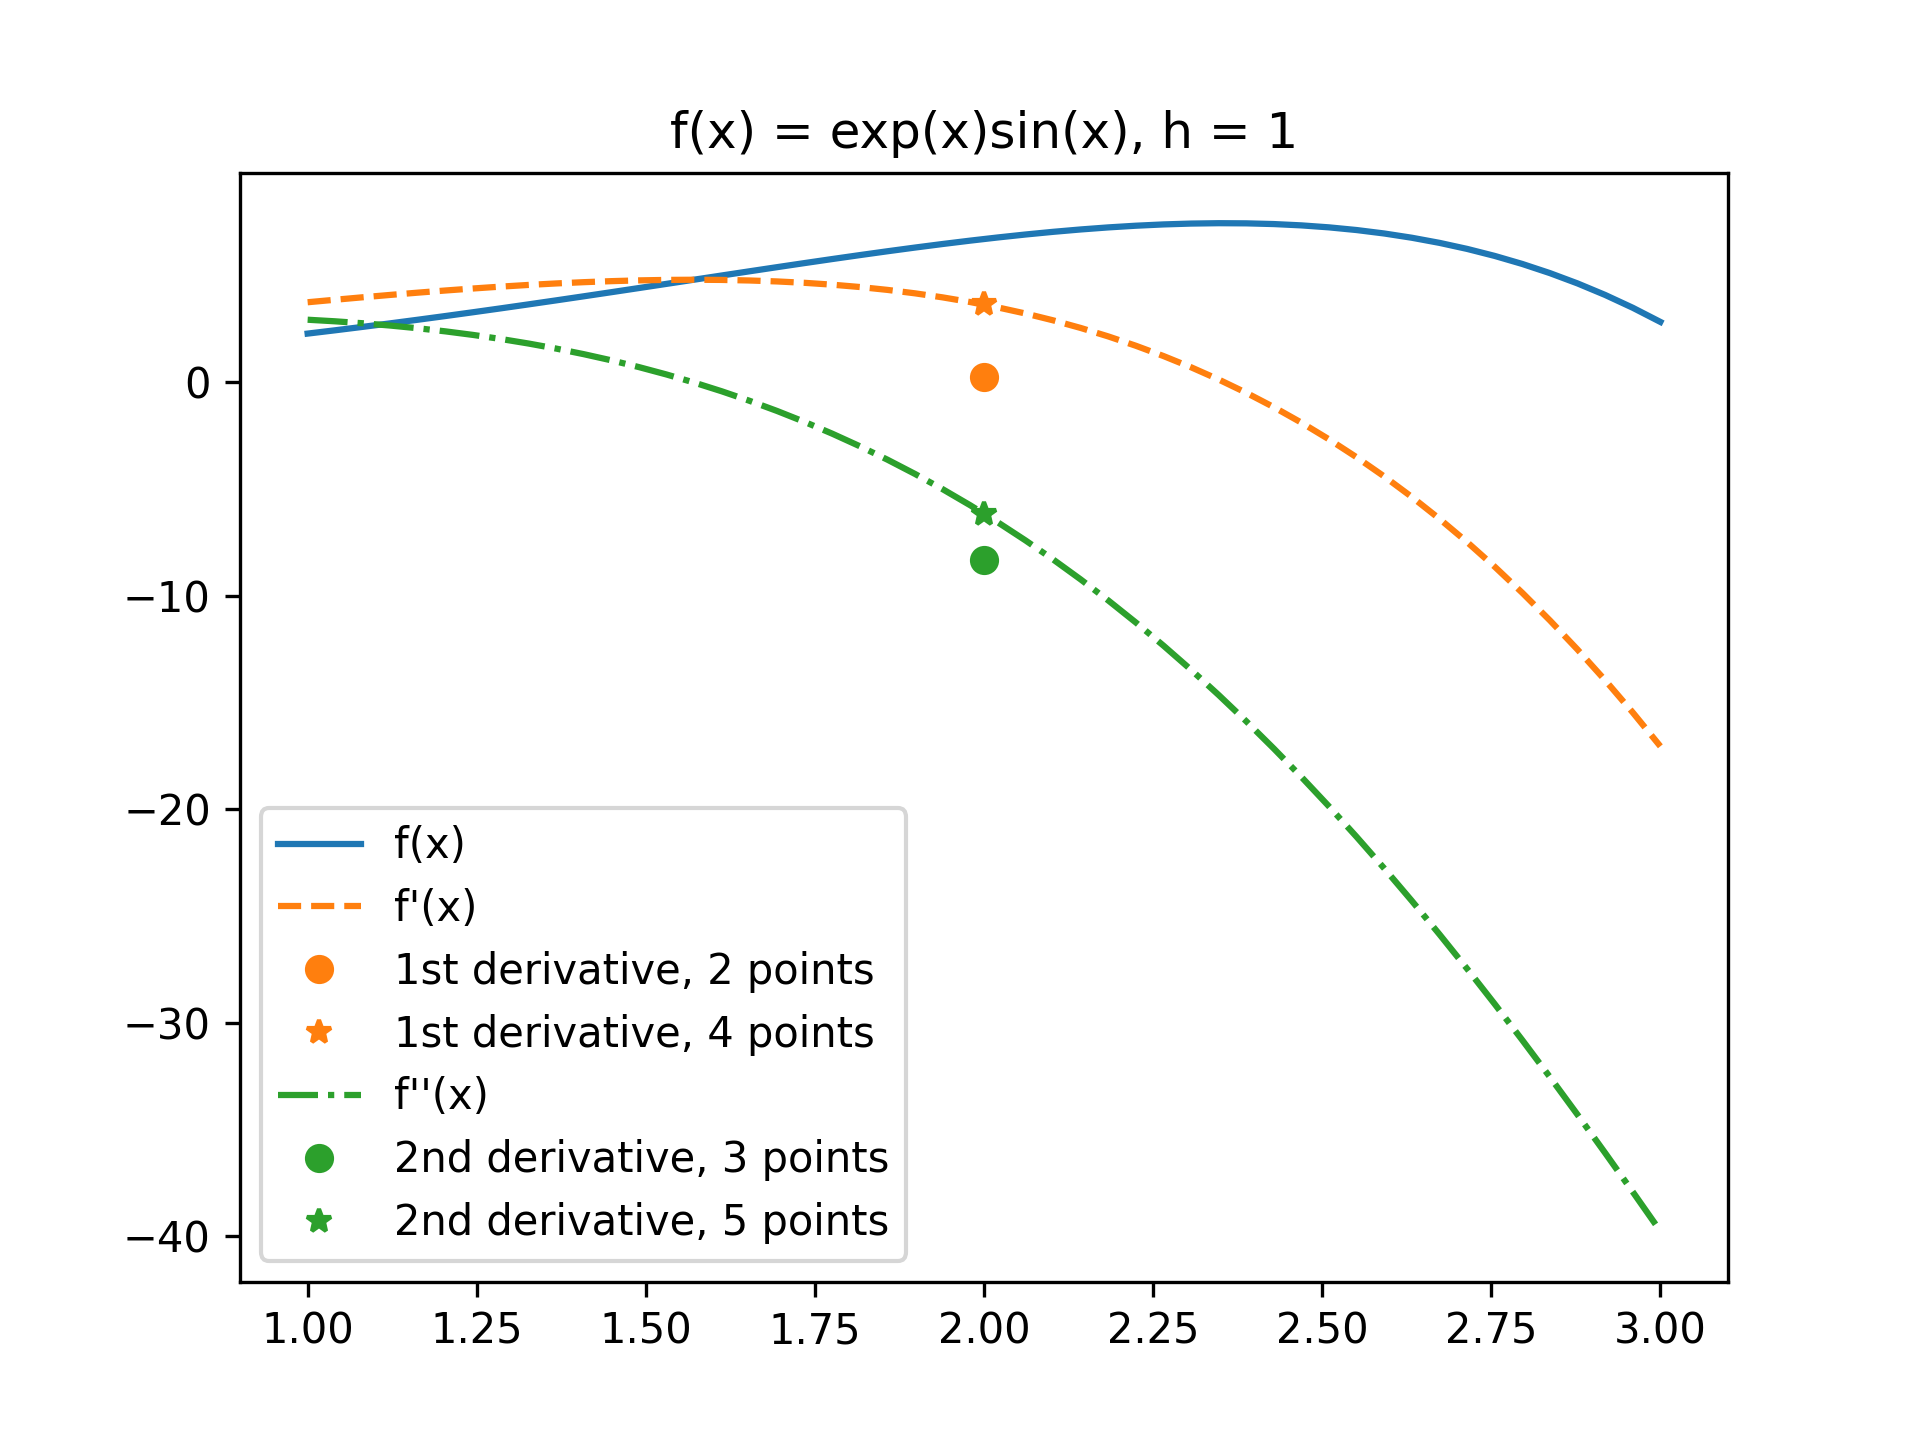
\includegraphics[width=.8\textwidth]{figs/q4.png}
  \captionof{figure}{Aproximação para 1a e 2a derivada.}
  \label{fig:q4}
\end{figure}
Considerando, por exemplo, $h=\Delta x = 1$ e
utilizando a aproximação obtida na Eq.\eqref{eq:leveque_coeffs} para $f'(x=2)$
e $f''(x=2)$, obtemos os seguintes valores para os casos solicitados

(i) Central com 2 e 3 pontos
obtemos os coeficientes 


(ii) Central com 4 e 5 pontos

caso desejemos plotar a dependência do erro de aproximação com relação ao passo dediscretização $h$, vide Fig.~\ref{fig:q4_error}, percebemos que as aproximações com mais pontos, 3 pontos para a primeira derivada e 5 pontos para a segunda, resultam em um erro menor independente do valor de $h$. Além disso, percebe-se que o valor de $h$ influencia positivamente o erro, com menores valores de $h$ resultando em erros menores, efeito observado independente do número de pontos.
\begin{figure}[h]
  \centering
  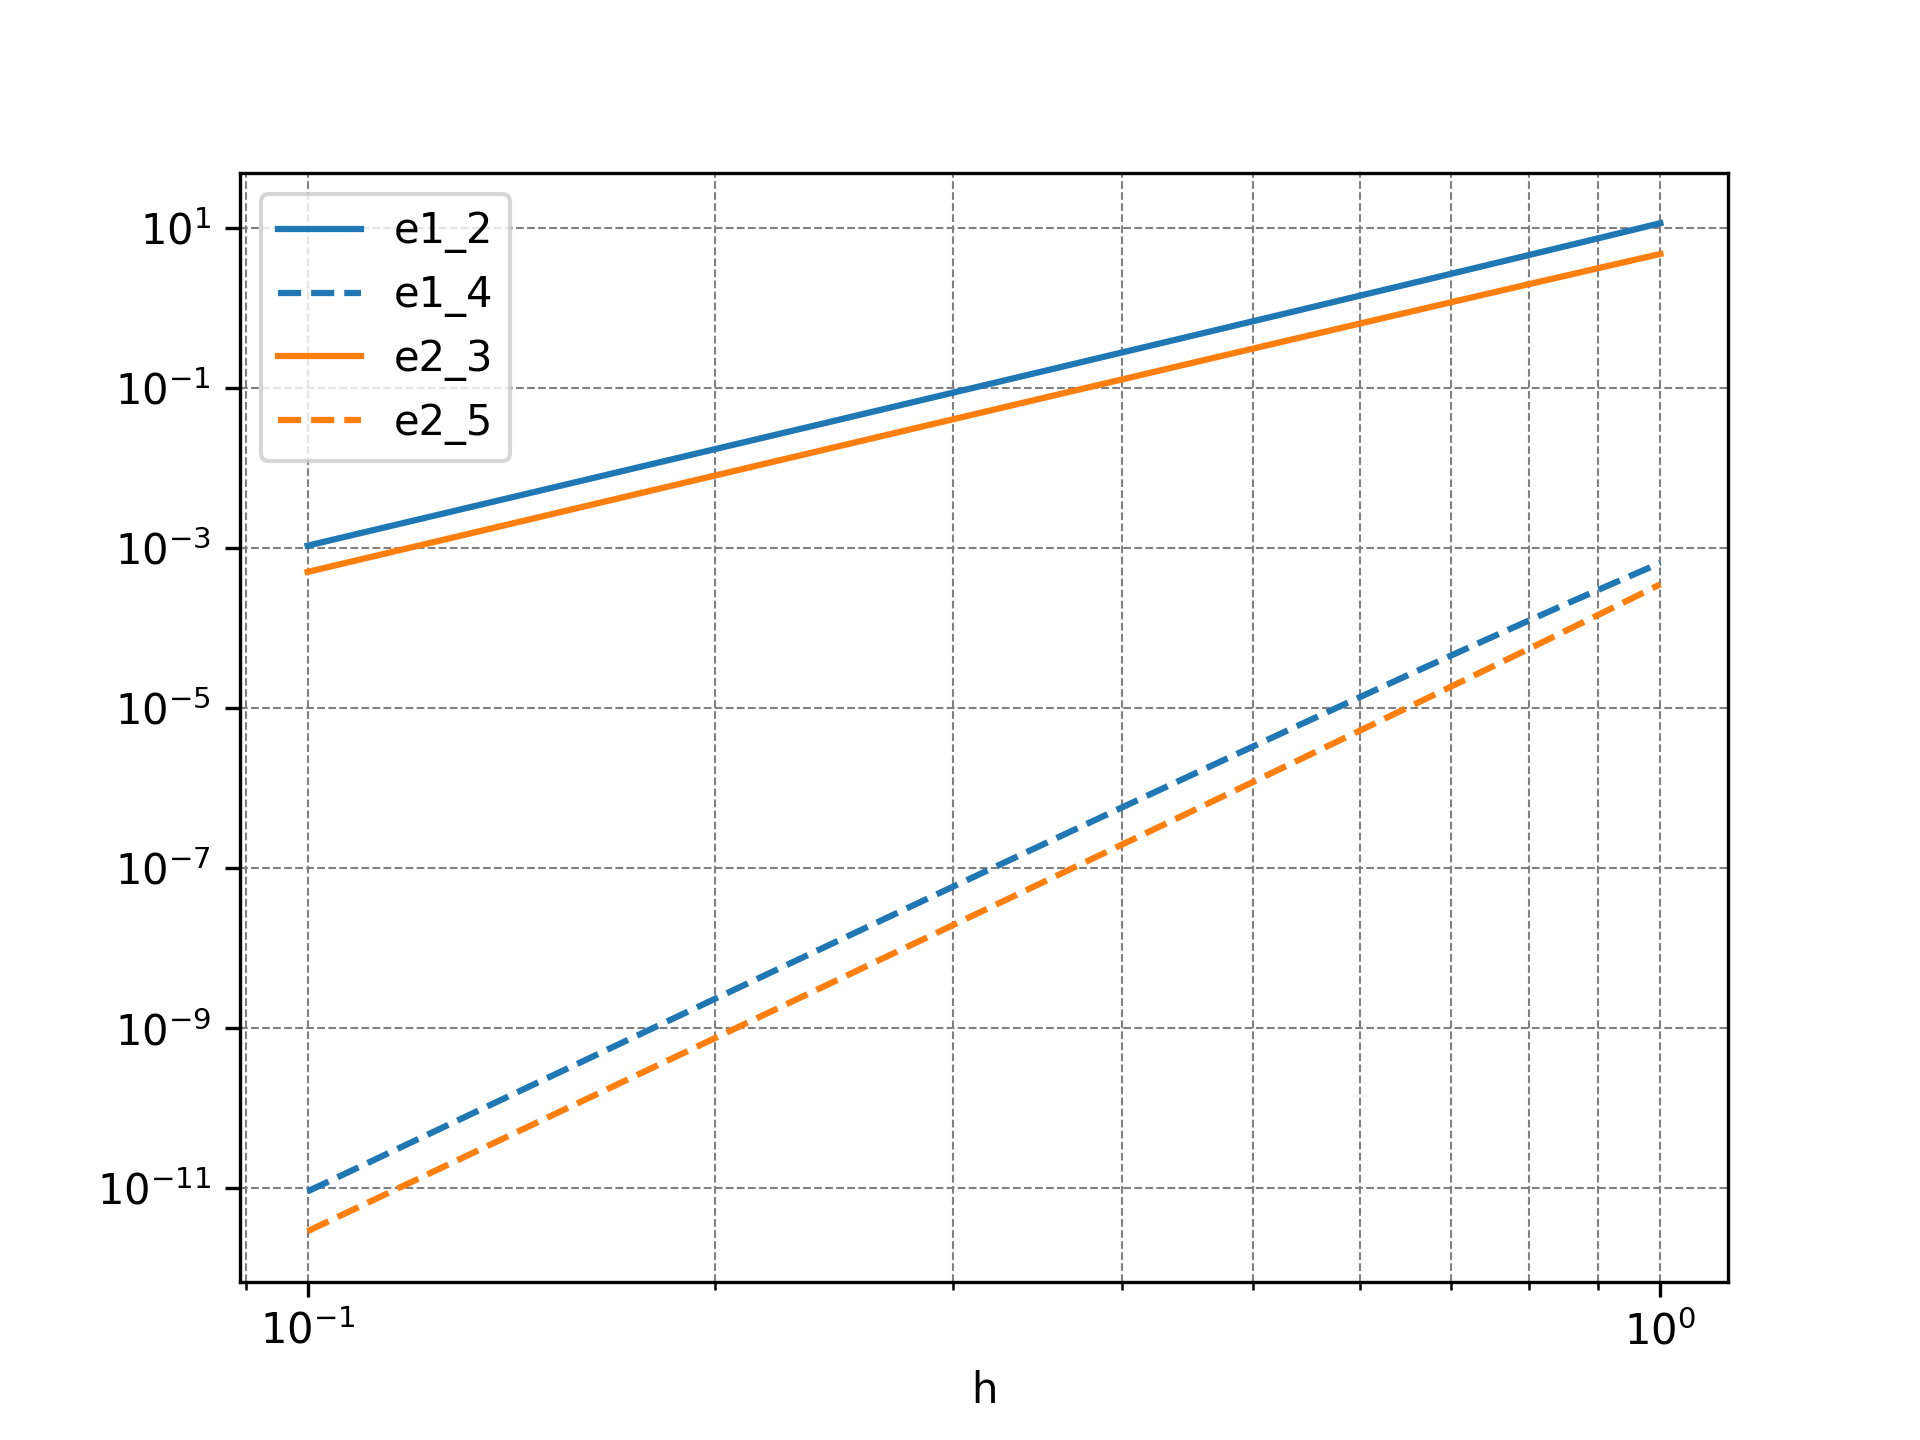
\includegraphics[width=.8\textwidth]{figs/q4_error.png}
  \captionof{figure}{Evolução do erro de aproximação com variação de $h$.}
  \label{fig:q4_error}
\end{figure}

\section{Questão 5}
Q5 took 12.47940993309021 seconds
\begin{figure}[h]
\centering
  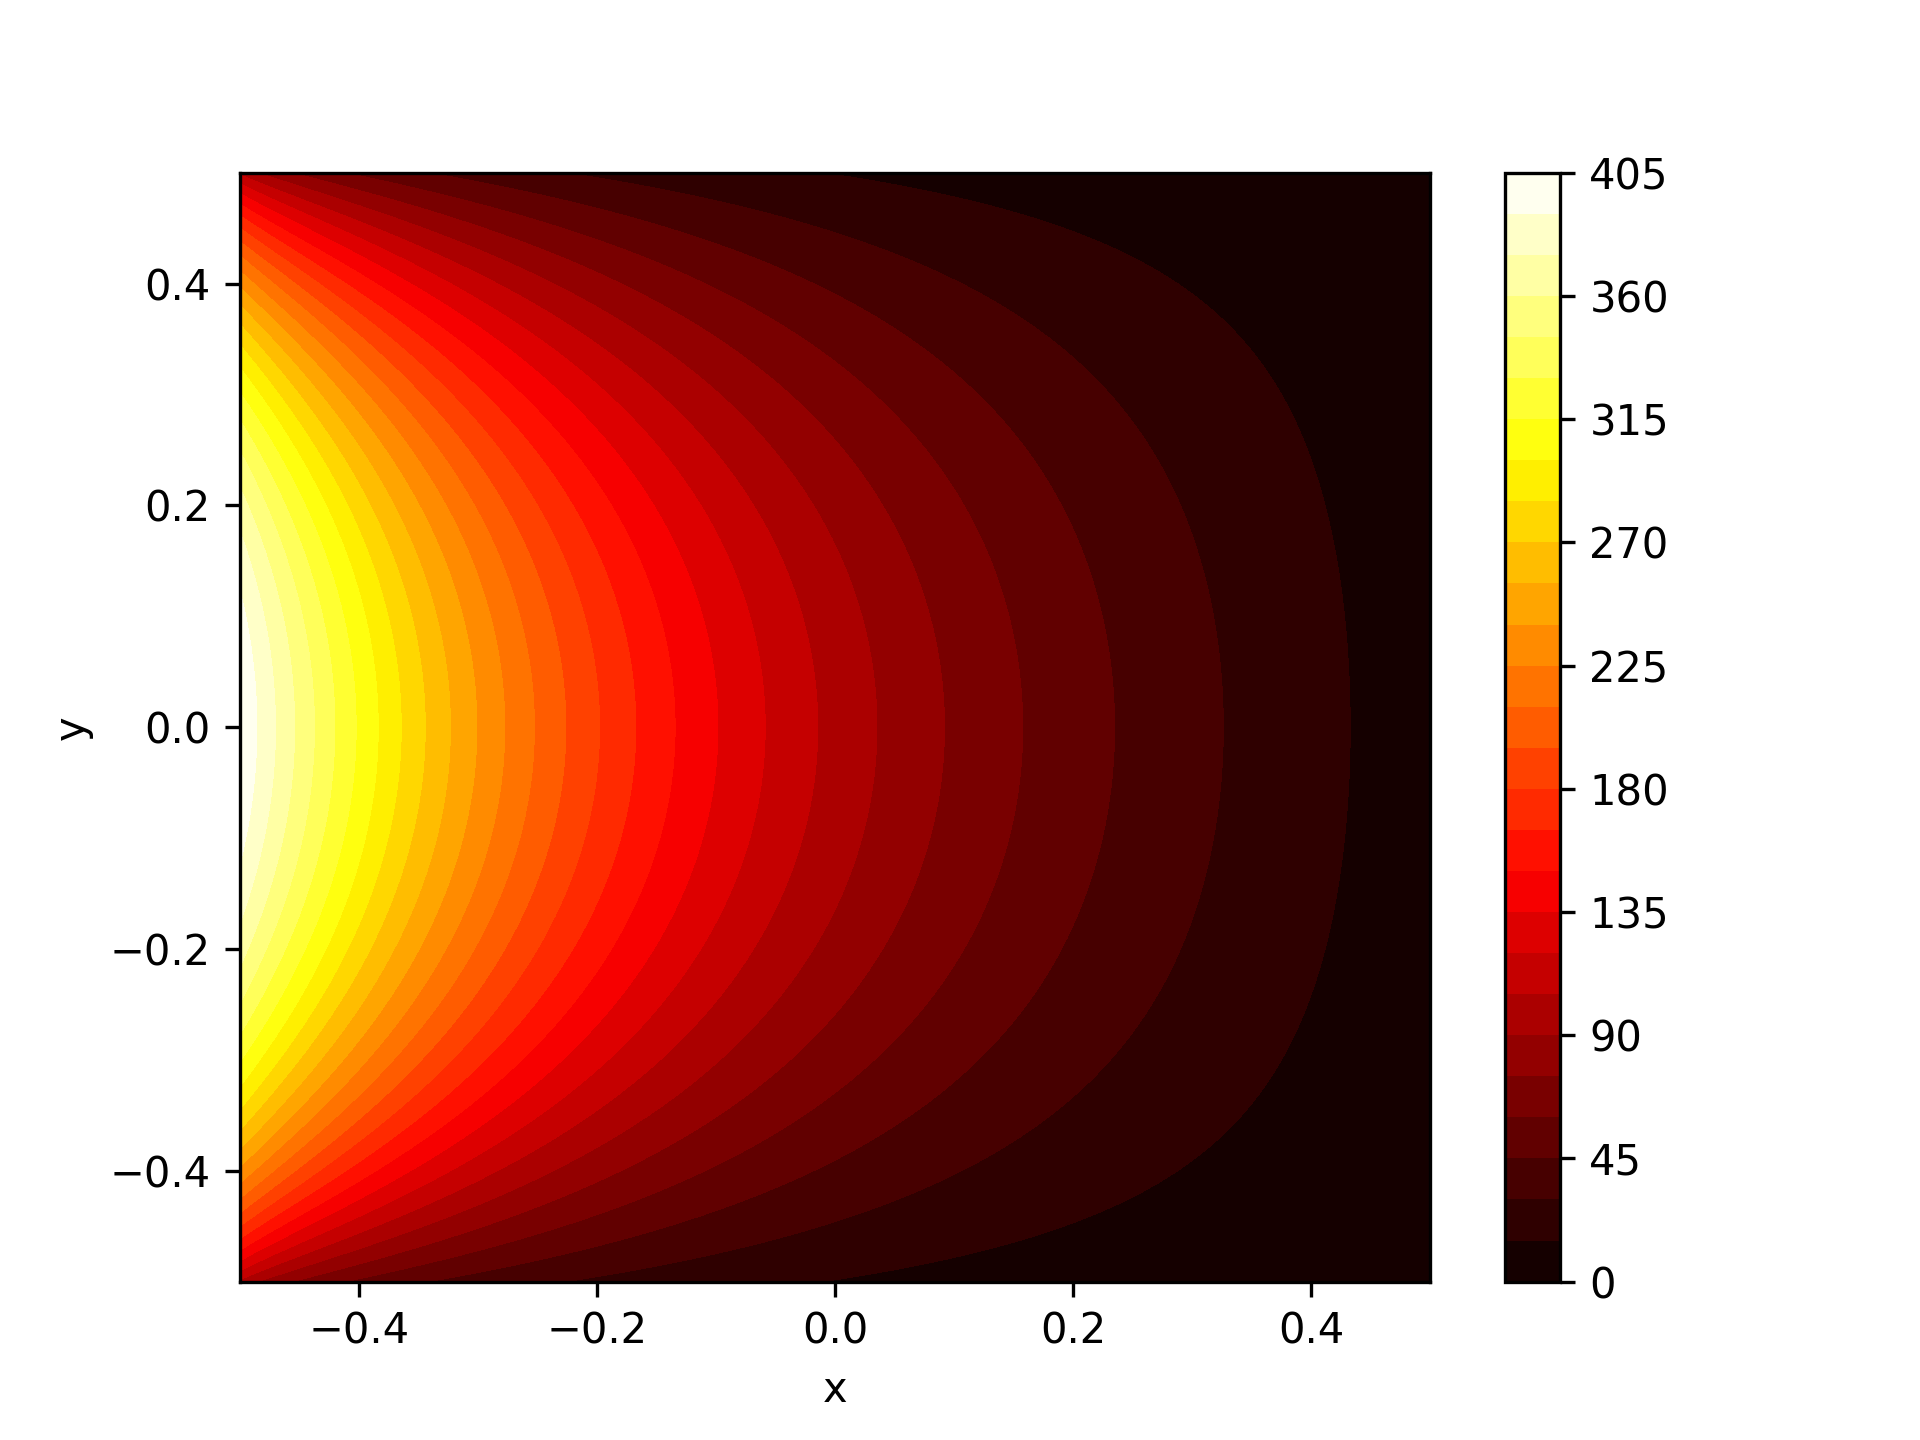
\includegraphics[width=.8\textwidth]{figs/q5_colorbar.png}
  \captionof{figure}{Heatmap para a solução explícita em $T=0$ segundos}
	\label{fig:q5_colobar}
\end{figure}

\section{Questão 6}

\begin{lstlisting}
## Input data
# Geometry and material properties
L = 1
lamb = 0.01
# Boudary conditions
q = 1
# Initial conditions
T0 = 1
# Final time
tend = 30

## Discretization
N = 50  # spatial
Nt = 3000  # temporal
x = np.linspace(0, L, N)
t = np.linspace(0, tend, Nt)
dx = x[1] - x[0]
dt = t[1] - t[0]

beta = lamb * dt / (dx**2)

T = np.zeros((N, Nt))
for k, tk in enumerate(t):
    if tk == 0:
        for i, xi in enumerate(x):
            T[i, k] = T0
    else:
        for i, xi in enumerate(x):
            if np.isclose(xi, 0):
                if t[k] <= 10:
                    T[i, k] = T[i, k - 1] + beta * (
                        2 * T[i + 1, k - 1] 
                        - 2 * T[i, k - 1] + 2 * dx * q
                    )
                else:
                    T[i, k] = T[i, k - 1] + beta * (
                        2 * T[i + 1, k - 1] - 2 * T[i, k - 1]
                    )
            elif np.isclose(xi, L):
                T[i, k] = T[i, k - 1] + beta * (2 * T[i - 1, k - 1]
                - 2 * T[i, k - 1])
            else:
                T[i, k] = T[i, k - 1] + beta * (
                    T[i - 1, k - 1] - 2 * T[i, k - 1] + T[i + 1, k - 1]
                )
\end{lstlisting}

\begin{lstlisting}
## Input data
# Geometry and material properties
L = 1
lamb = 0.01
# Boudary conditions
q = 1
# Initial conditions
T0 = 1
# Final time
tend = 30

## Discretization
N = 50  # spatial
Nt = 3000  # temporal
x = np.linspace(0, L, N)
t = np.linspace(0, tend, Nt)
dx = x[1] - x[0]
dt = t[1] - t[0]

beta = lamb * dt / (dx**2)

T = np.zeros((N, Nt))

# Matrix A assembly
A = np.zeros((N, N))

for i, xi in enumerate(x):
    if np.isclose(xi, 0):
        A[i, i] = 2 * beta + 1
        A[i, i + 1] = -2 * beta
    elif np.isclose(xi, L):
        A[i, i - 1] = -2 * beta
        A[i, i] = 2 * beta + 1
    else:
        A[i, i - 1] = -beta
        A[i, i + 1] = -beta
        A[i, i] = 2 * beta + 1

# print(A)

b = np.zeros(N)
# Solution
for k, tk in enumerate(t):
    if tk == 0:
        T[:, k] = T0
    else:
        b = list(T[:, k - 1])
        if t[k] <= 10:
            b[0] = b[0] + 2 * beta * dx * q
            T[:, k] = np.linalg.solve(A, b)
        else:
            T[:, k] = np.linalg.solve(A, b)
\end{lstlisting}

Q6a took 8.867920160293579 seconds
Q6b took 0.04085826873779297 seconds

Quanto à discretização adotada: 
para as derivadas no espaço, foi usada a aproximação de derivada central de 3 pontos e para as derivadas no tempo, aproximação de dois pontos.

Para aplicar as condições de contorno, foram utilizados pontos fantasma nas aproximações das derivadas espaciais, já que se tratavam de condições de contorno de Neumann.

\begin{figure}[h]
\centering
     \begin{subfigure}[b]{0.49\textwidth}
         \centering
         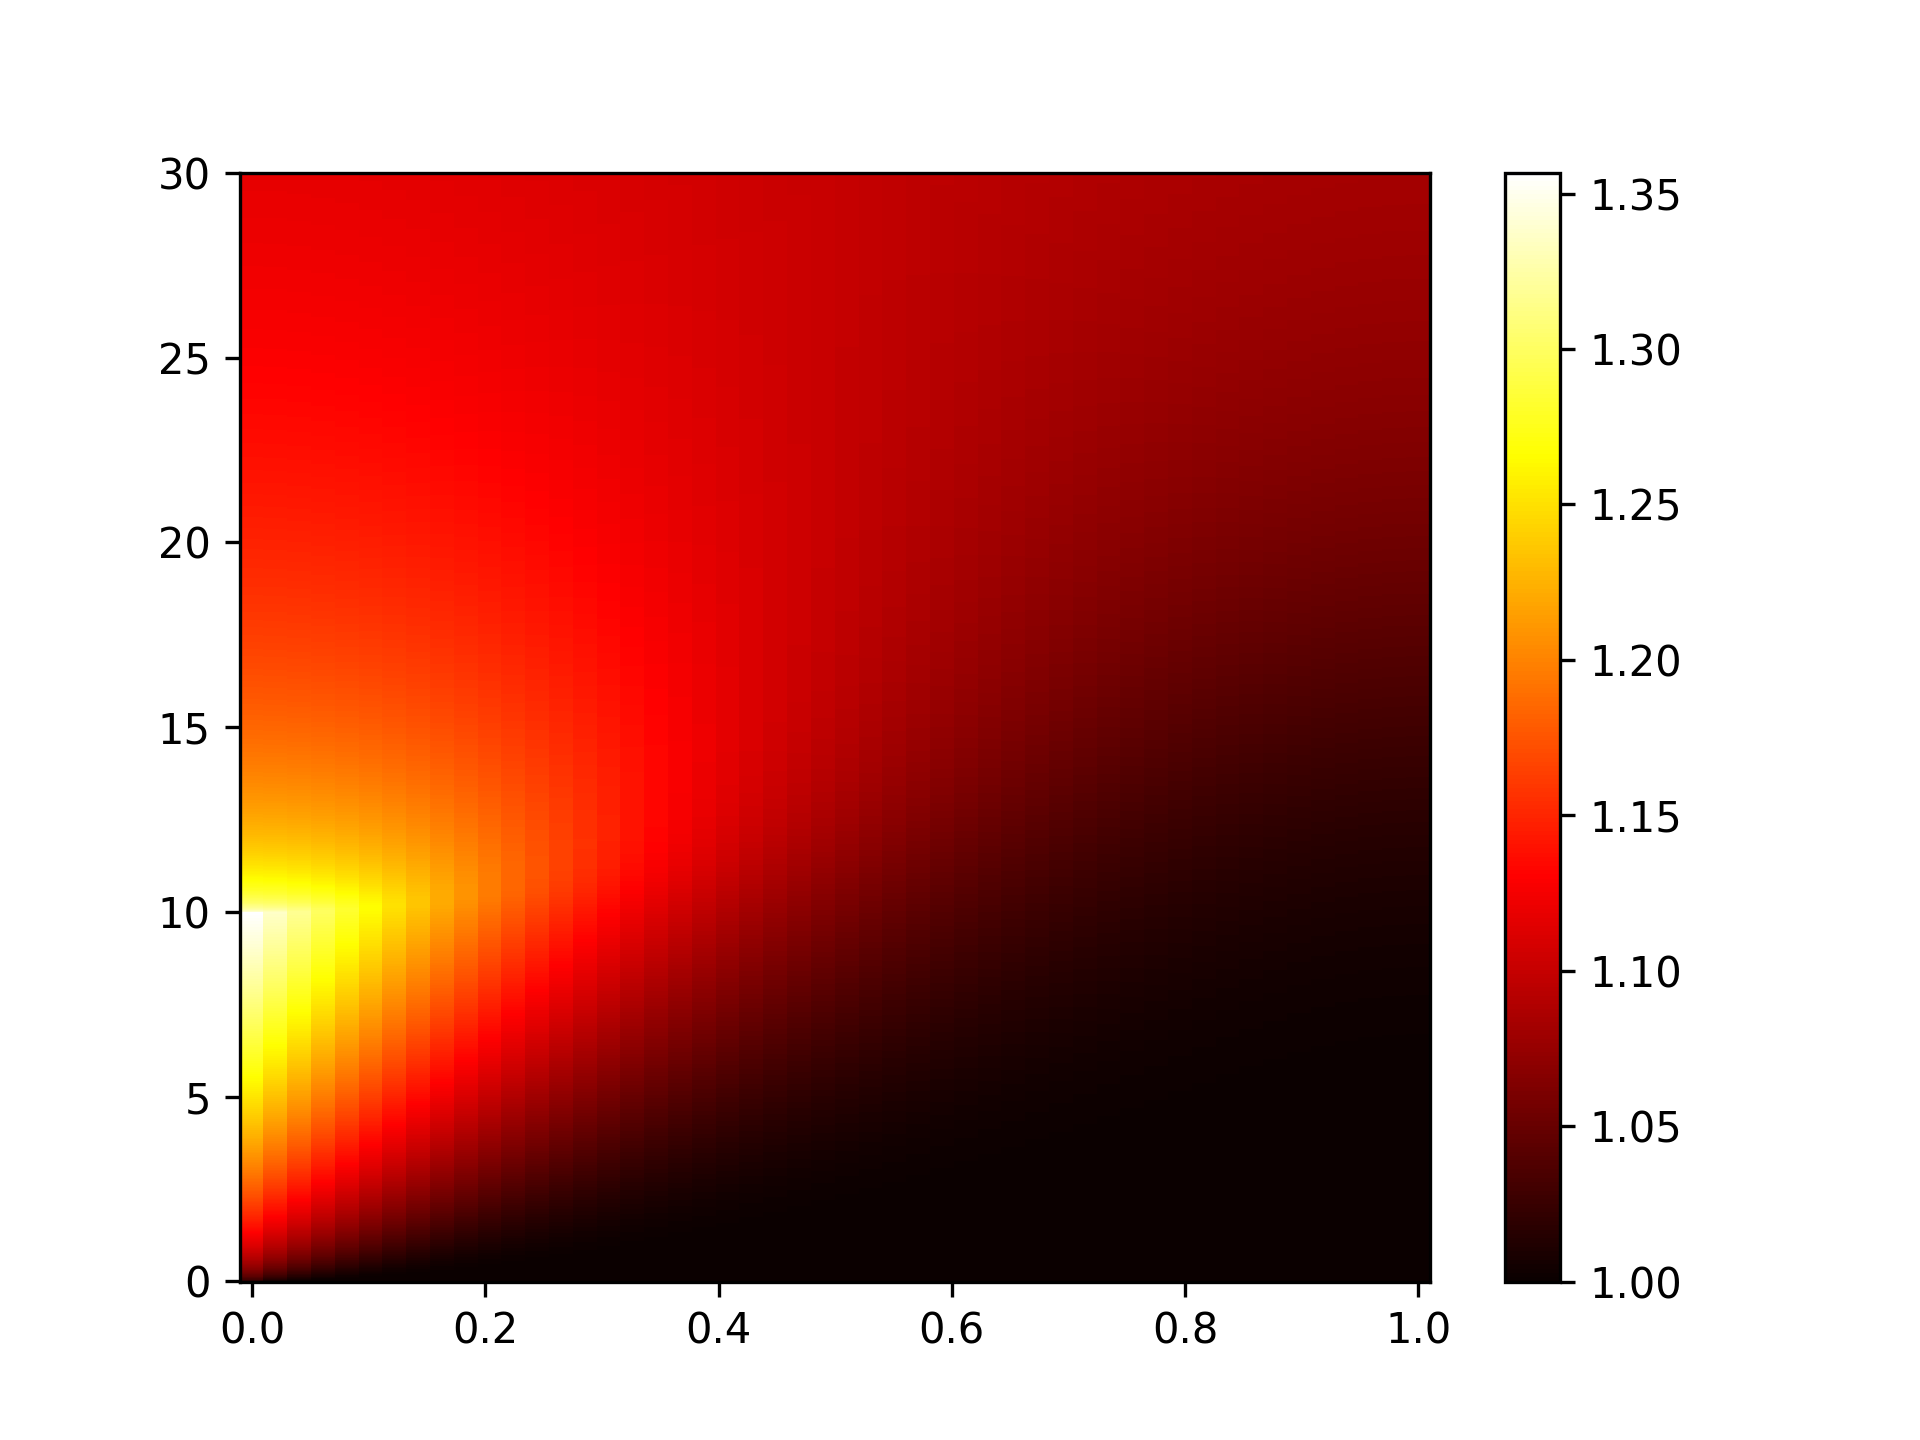
\includegraphics[width=\textwidth]{figs/q6a_colormap.png}
         \caption{ solução explícita}
	\label{fig:q6a_colobar}
     \end{subfigure}
     \hfill
     \begin{subfigure}[b]{0.49\textwidth}
         \centering
         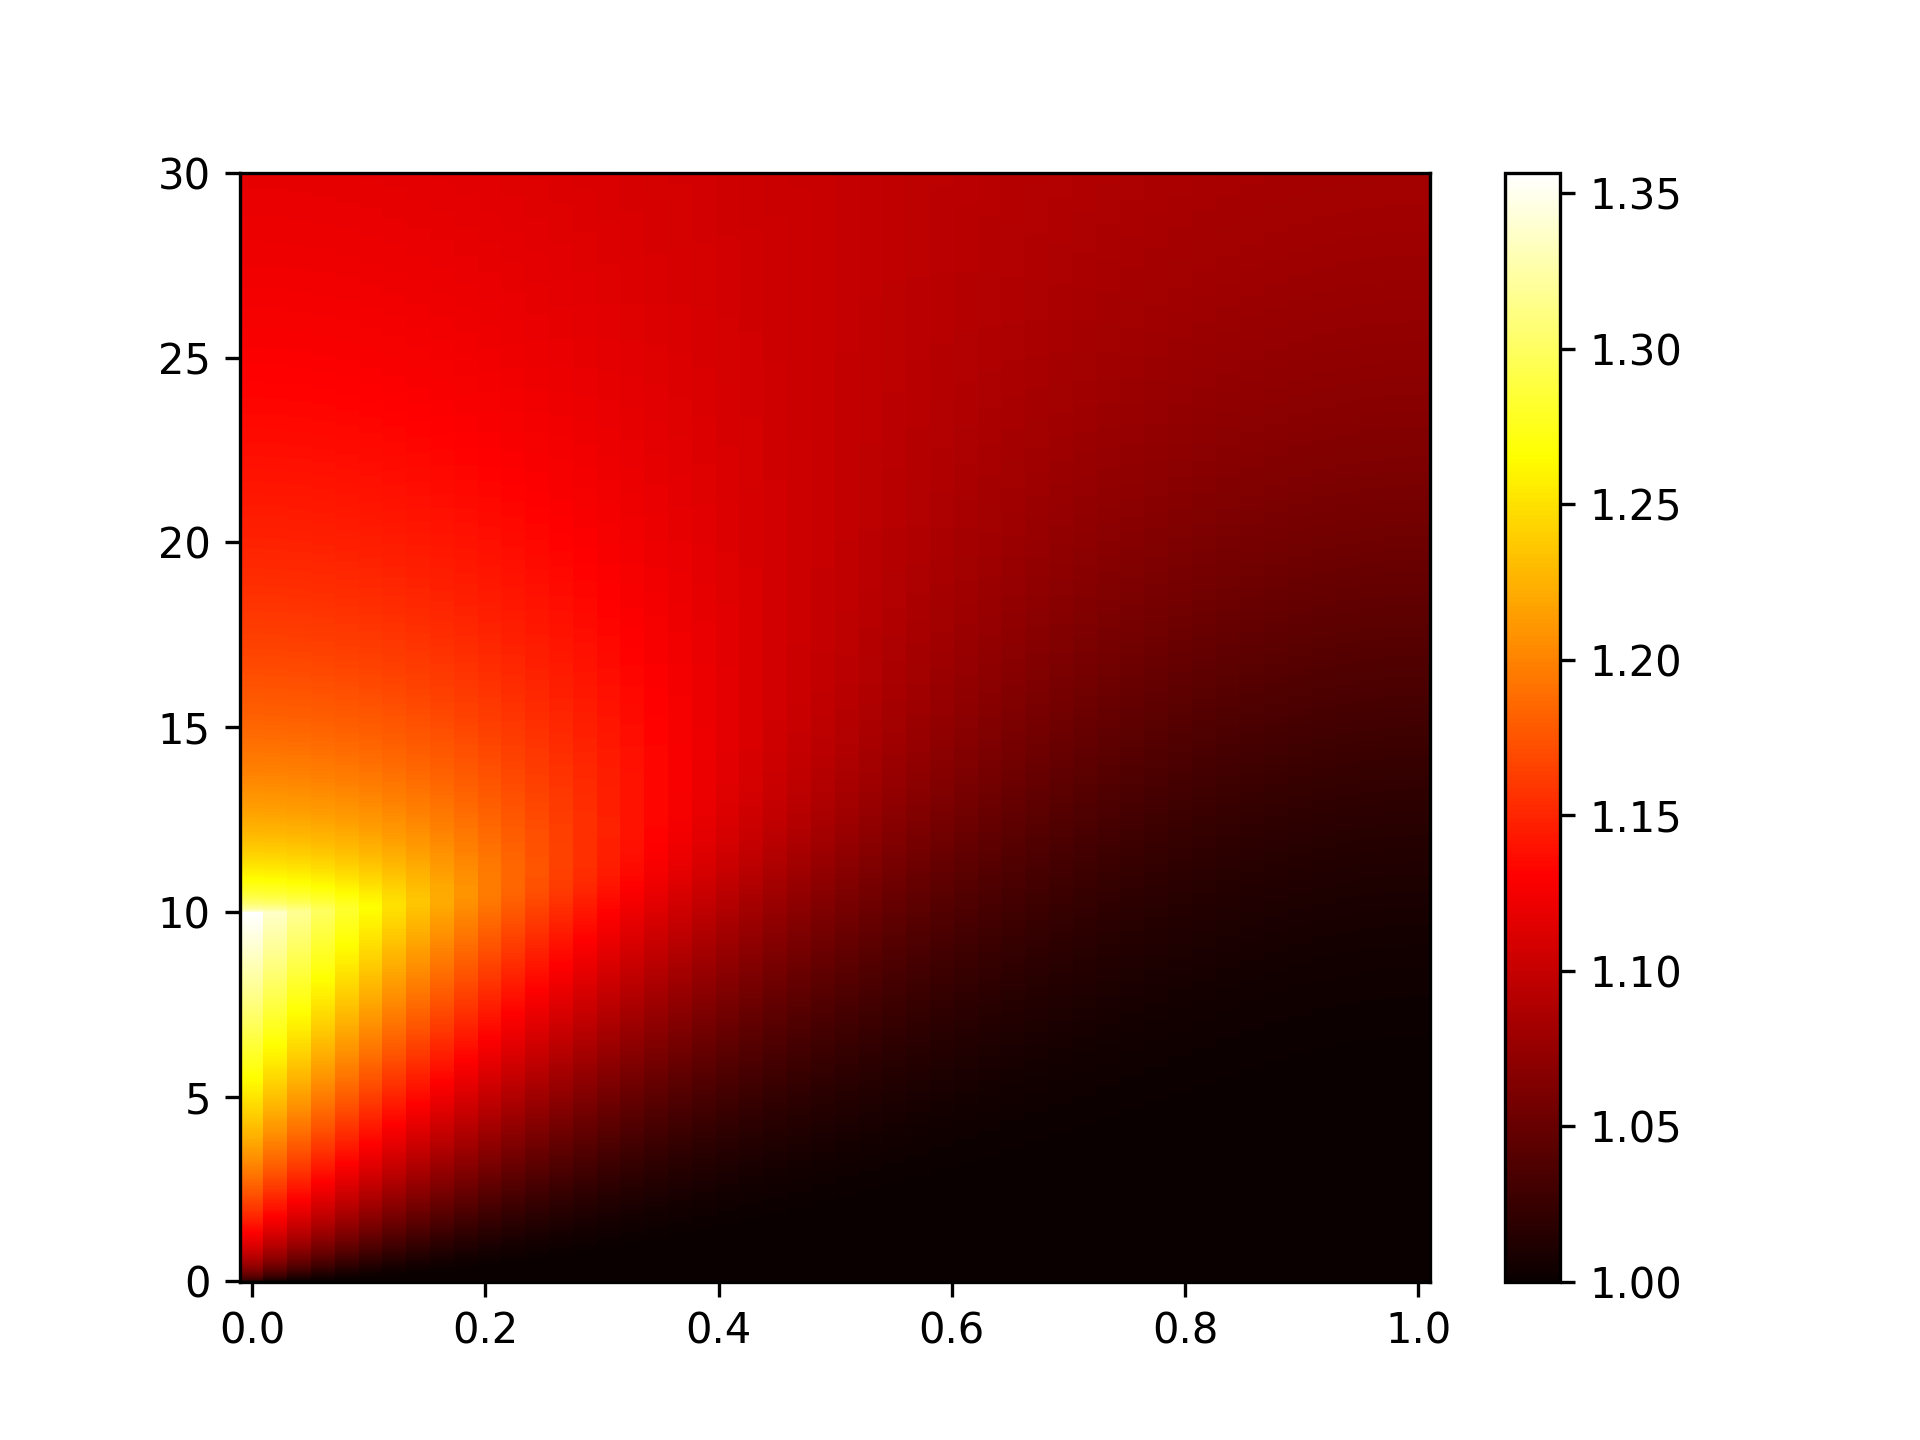
\includegraphics[width=\textwidth]{figs/q6b_colormap.png}
         \caption{solução implícita}
	\label{fig:q6b_colobar}
     \end{subfigure}
\caption{Colobar para Questão 6}
\end{figure}

\begin{figure}[h]
\centering
     \begin{subfigure}[b]{0.49\textwidth}
         \centering
         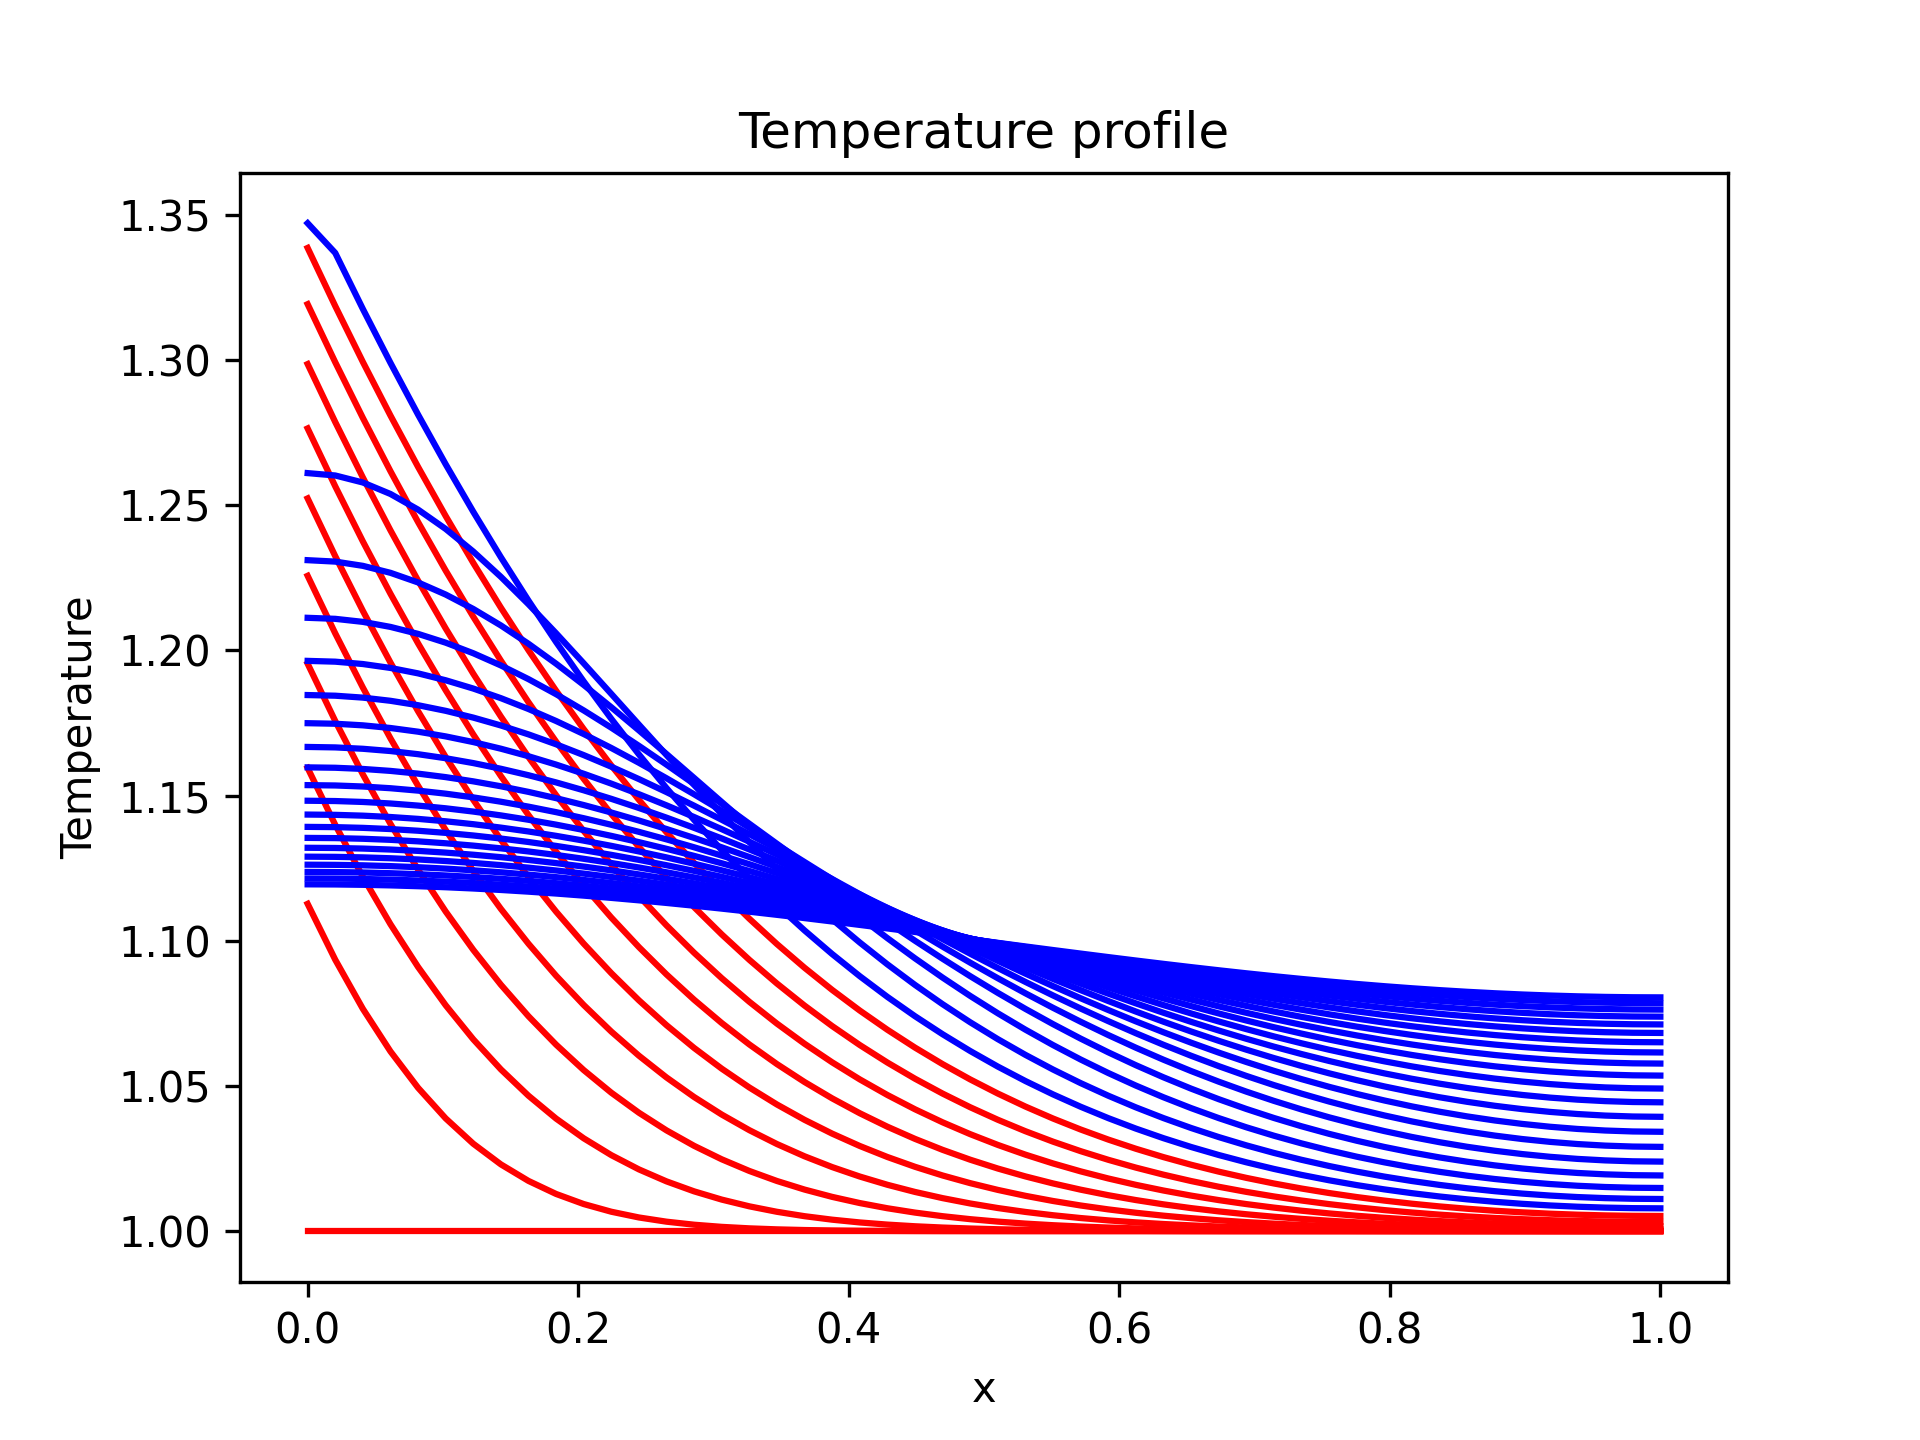
\includegraphics[width=\textwidth]{figs/q6a_temperature_profile.png}
         \caption{ solução explícita}
	\label{fig:q6a_temperature_profile}
     \end{subfigure}
     \hfill
     \begin{subfigure}[b]{0.49\textwidth}
         \centering
         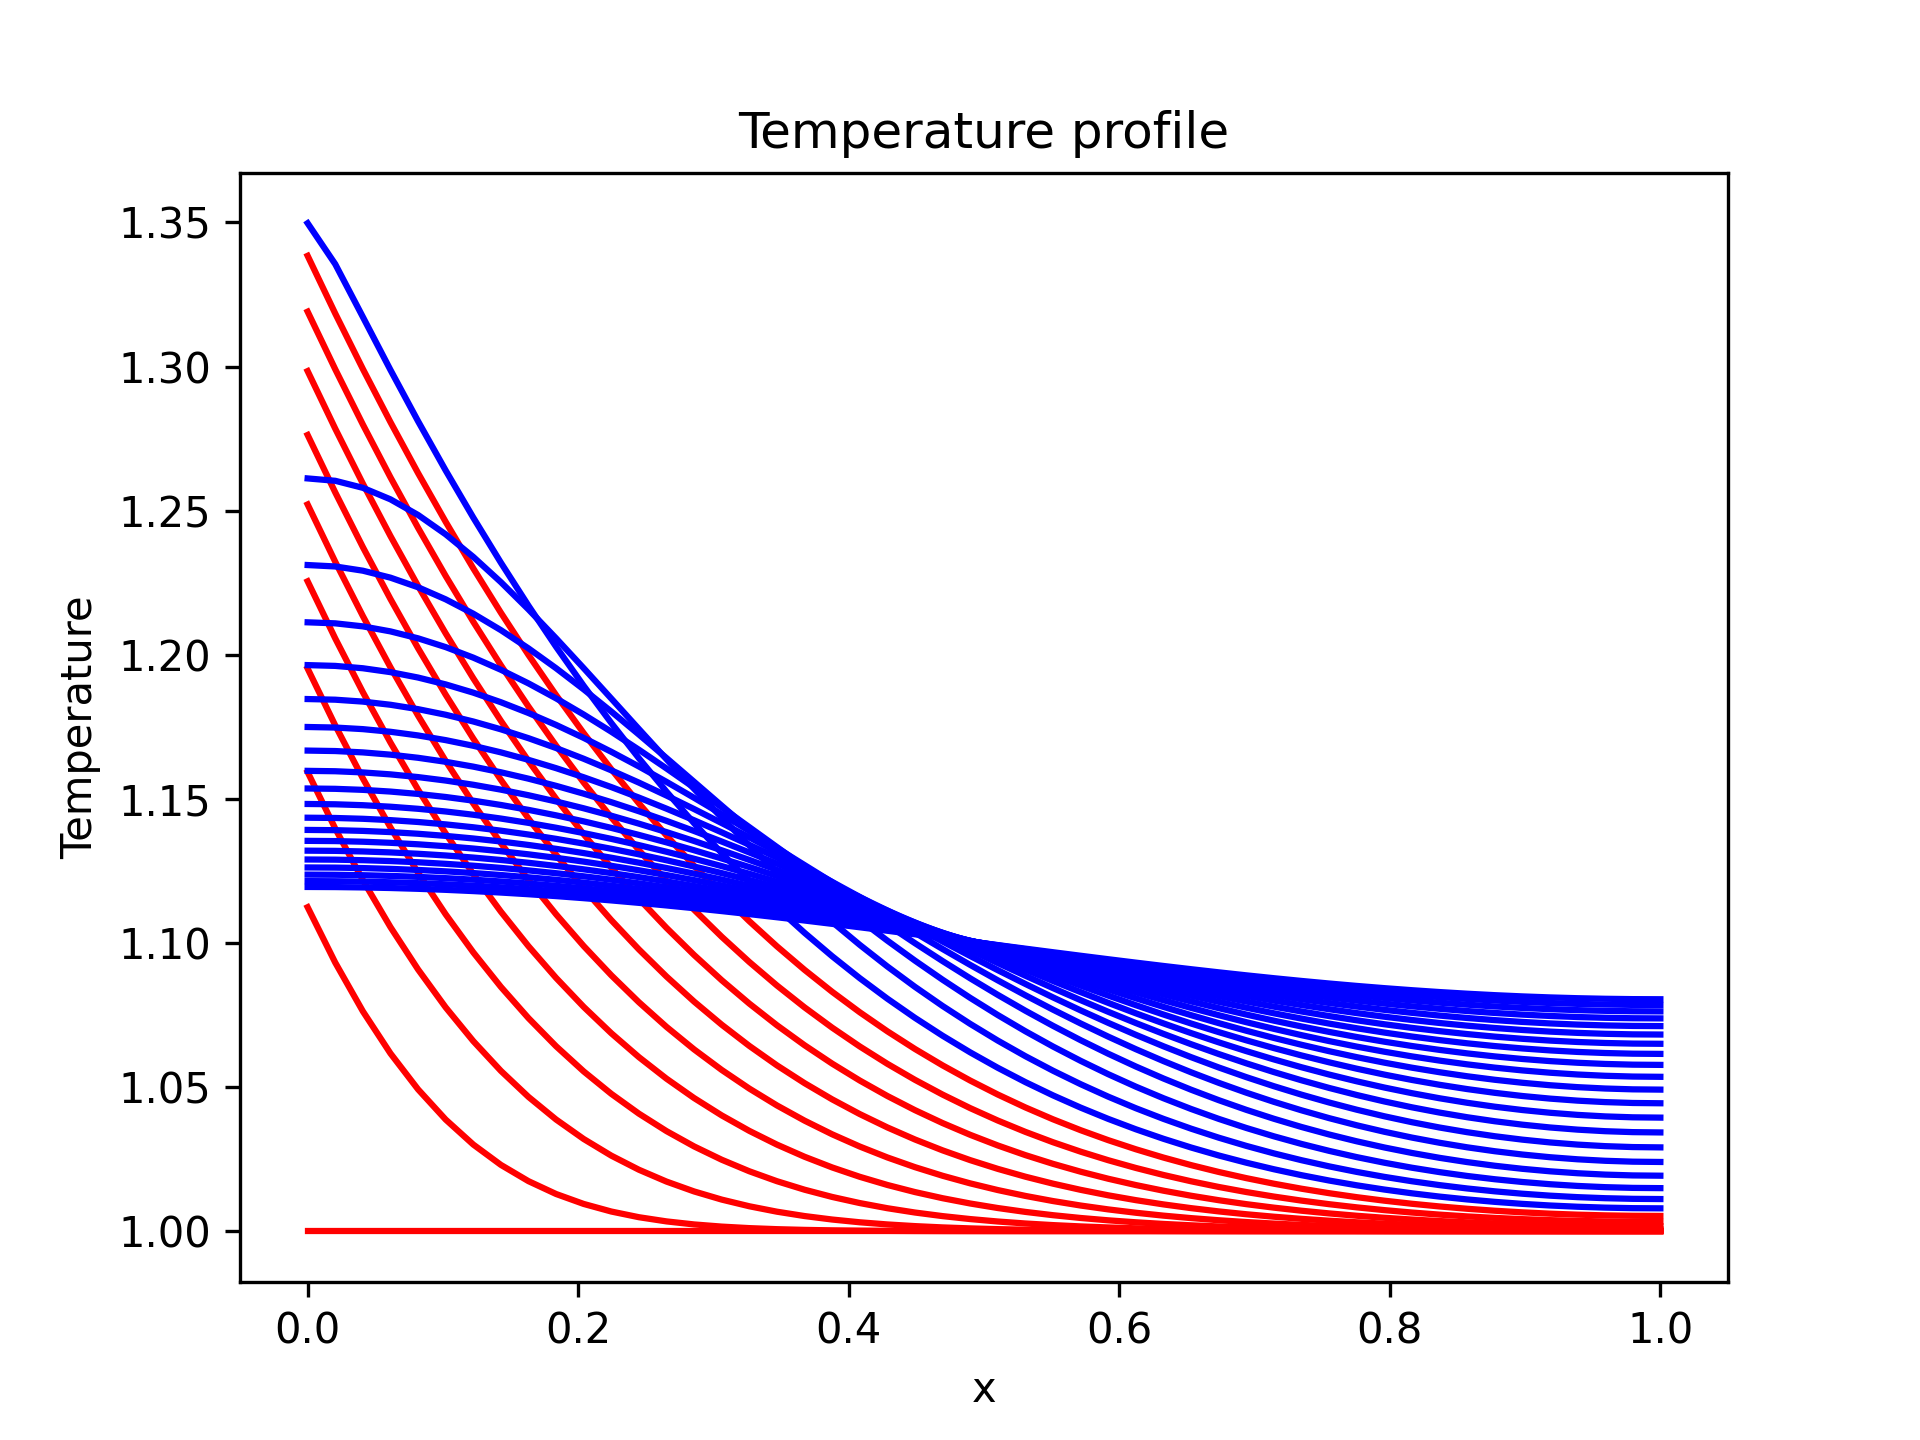
\includegraphics[width=\textwidth]{figs/q6b_temperature_profile.png}
         \caption{solução implícita}
	\label{fig:q6b_temperature_profile}
     \end{subfigure}
\caption{Perfis de temperature Questão 6}
\end{figure}

\begin{figure}[h]
\centering
     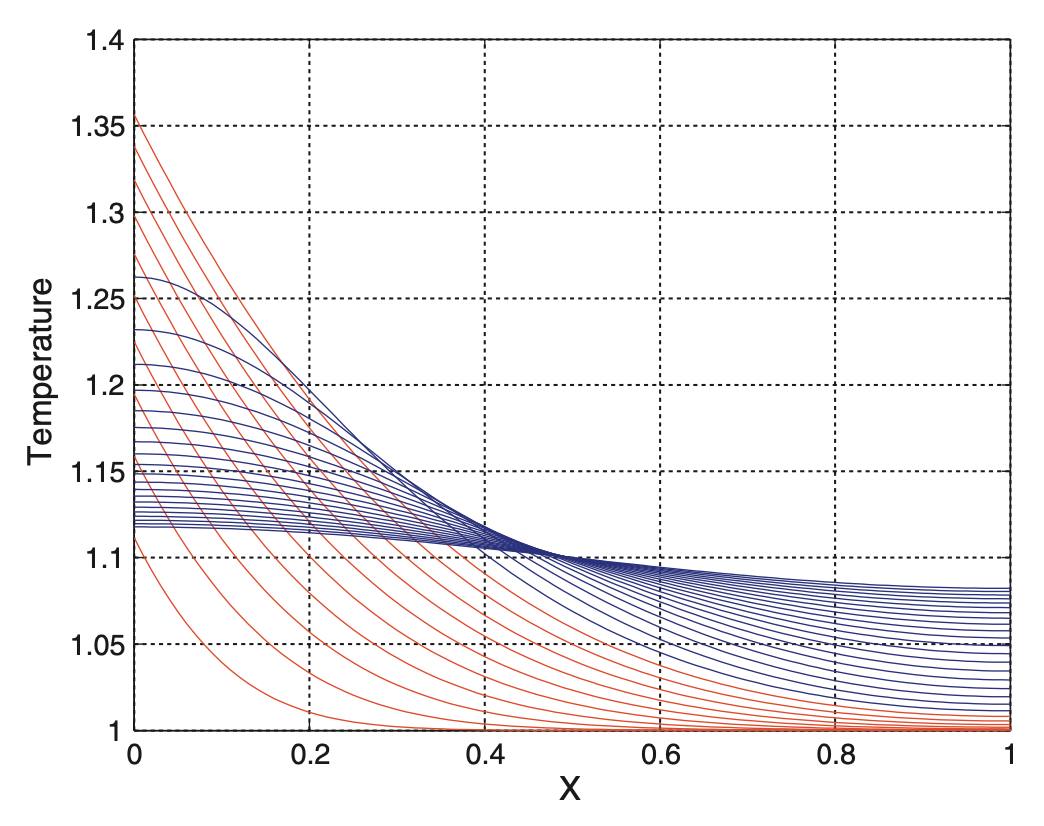
\includegraphics[width=\textwidth]{figs/chinesta_fig1.png}
     \caption{Figura 01 de \cite{chinesta}, "
Temperature profiles corresponding to the source term (13) at discrete times
$t_m =m$,for $m=1,2,...,30$. The red curves correspond to the heating stagel up to $t=10$, while the blue curves for $t > 10$ illustrate the heat transfer by conduction from the
warmest zones towards the coldest ones. (For interpretation of the references to
    color in this figure legend, the reader is referred to the web version of the article.)"}
    \label{fig:chinesta}
\end{figure}


\section{Questão 7}

Q7a took 2.9745030403137207 seconds
Q7b took 4.0168750286102295 seconds

Para a questão 7, as discretizações e condições de contorno adotadas foram as mesmas da questão 6:
para as derivadas no espaço, foi usada a aproximação de derivada central de 3 pontos e para as derivadas no tempo, aproximação de dois pontos.

Para aplicar as condições de contorno, foram utilizados pontos fantasma nas aproximações das derivadas espaciais, já que se tratavam de condições de contorno de Neumann.
\begin{figure}[h]
\centering
     \begin{subfigure}[b]{0.49\textwidth}
         \centering
         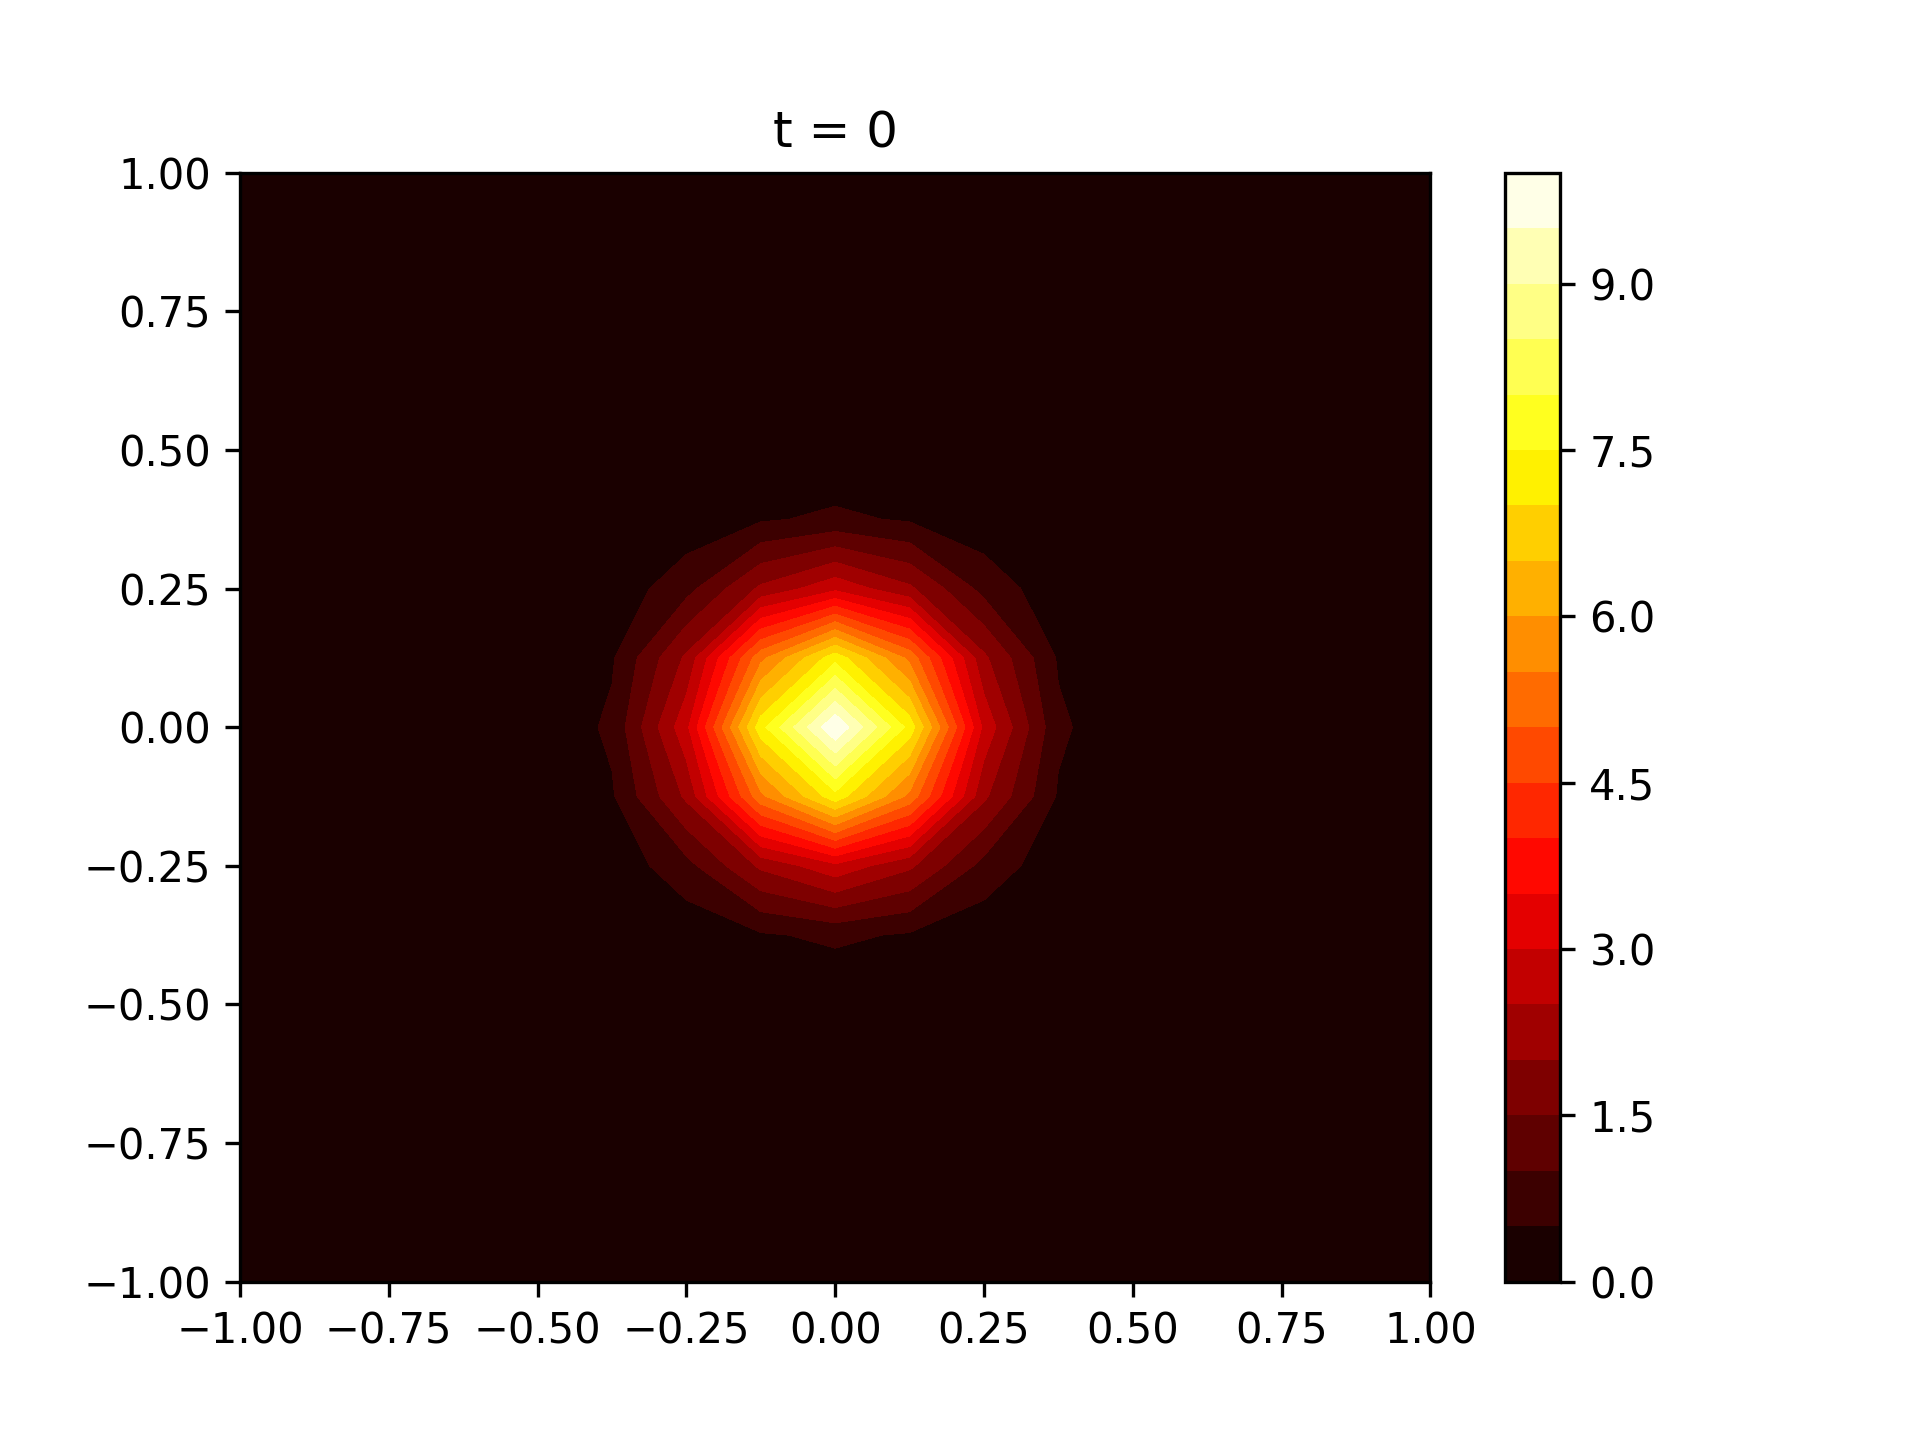
\includegraphics[width=\textwidth]{figs/q7a_heatmap_t0.png}
         \caption{$T=0~s$, solução explícita}
	\label{fig:q7a_heatmap_t0}
     \end{subfigure}
     \hfill
     \begin{subfigure}[b]{0.49\textwidth}
         \centering
     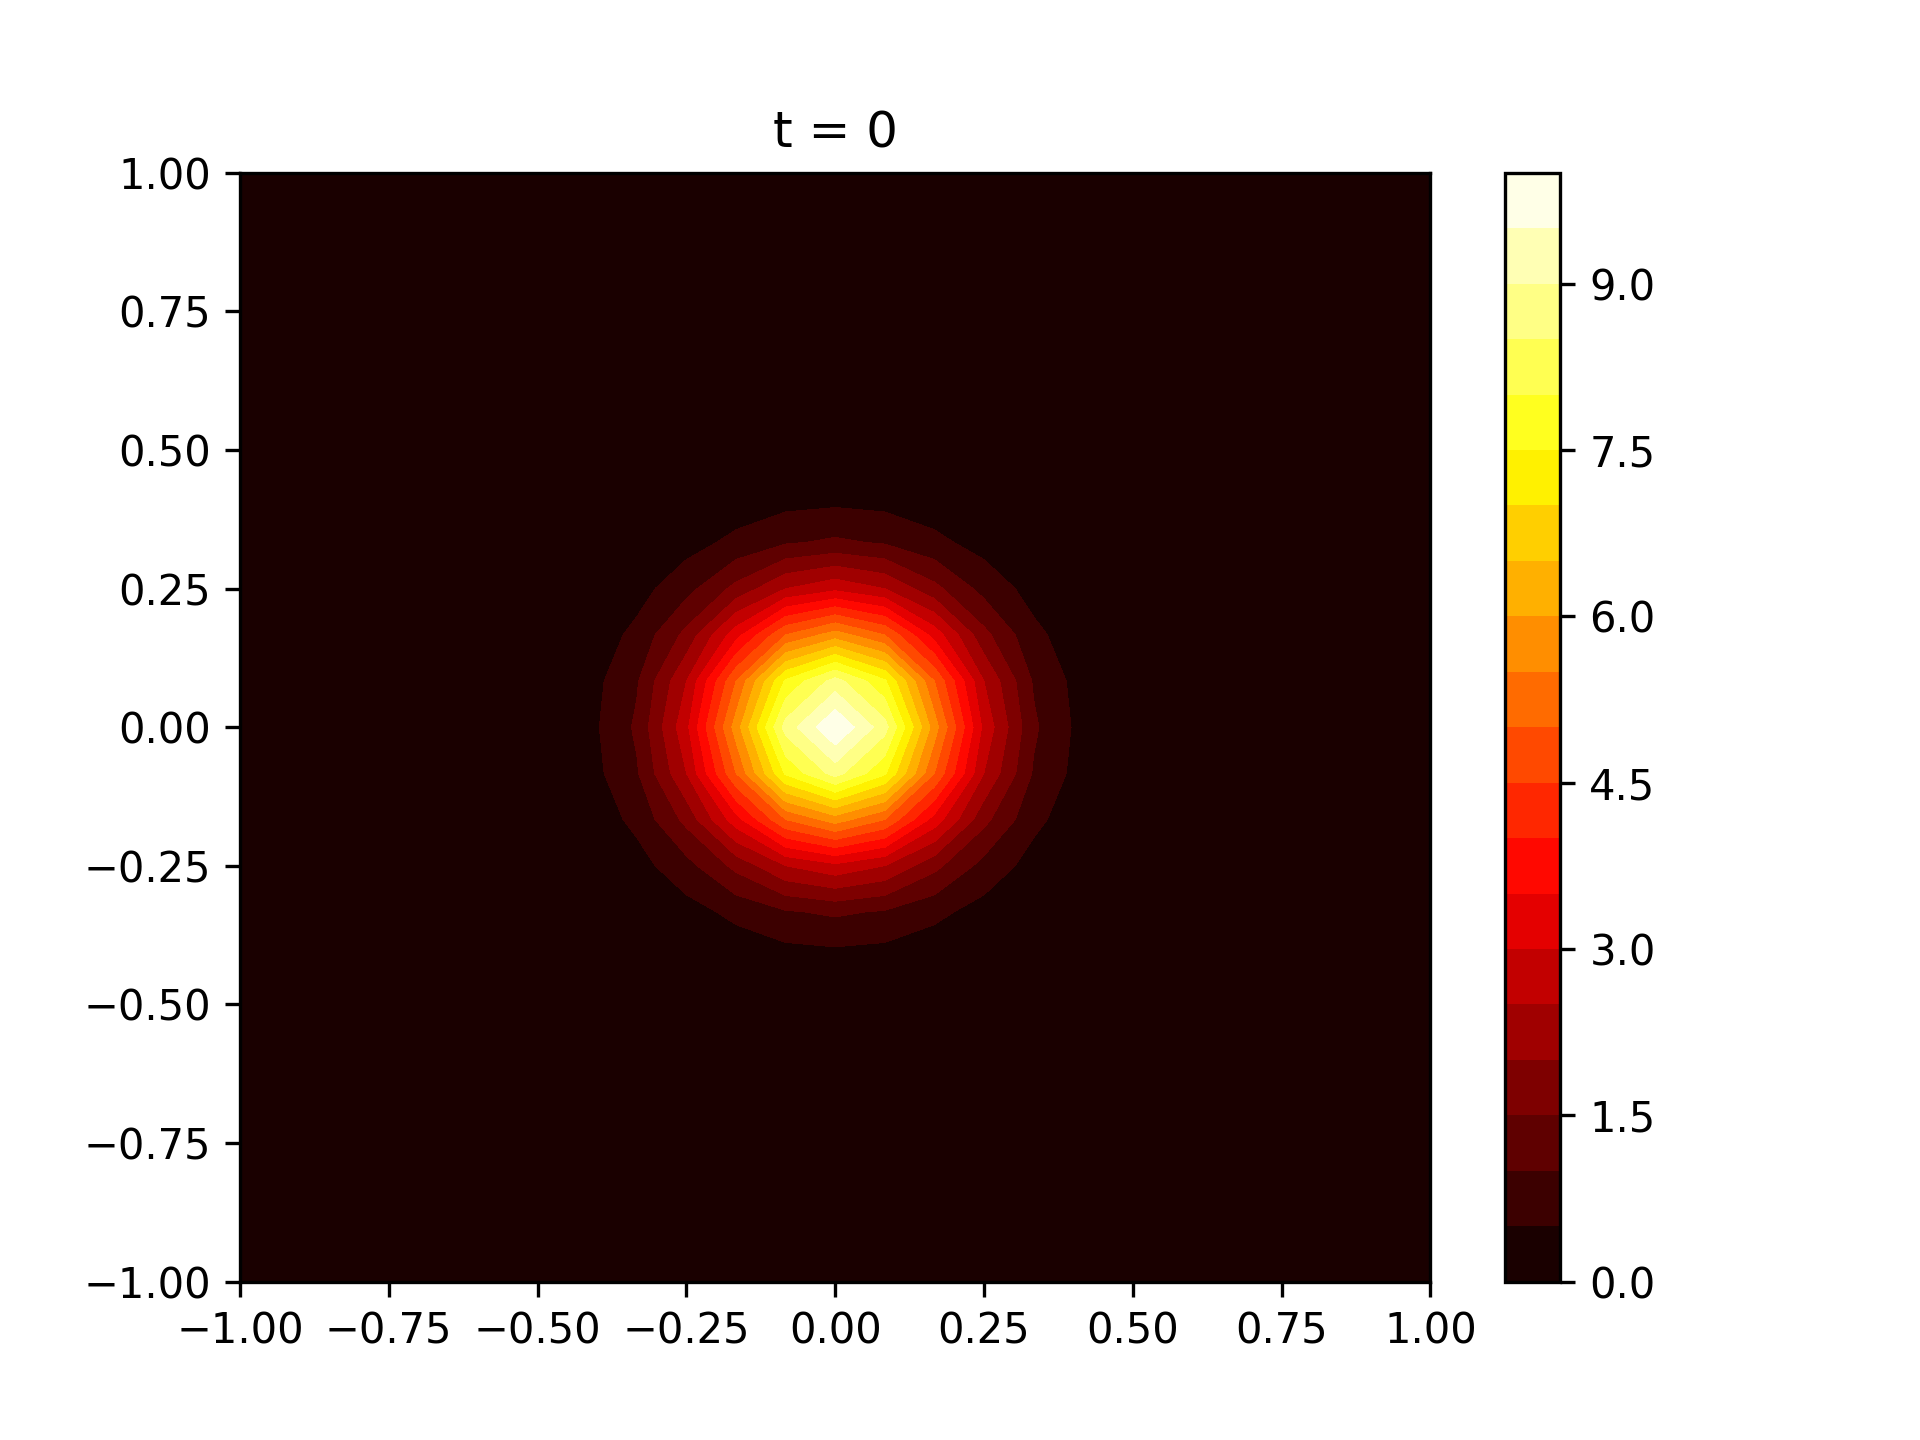
\includegraphics[width=\textwidth]{figs/q7b_heatmap_t0.png}
         \caption{$T=0~s$, solução implícita}
	\label{fig:q7b_heatmap_t0}
     \end{subfigure}
	\caption{Distribuição de temperatura inicial para a questão 7.}
\end{figure}

\begin{figure}[h]
     \begin{subfigure}[b]{0.49\textwidth}
         \centering
         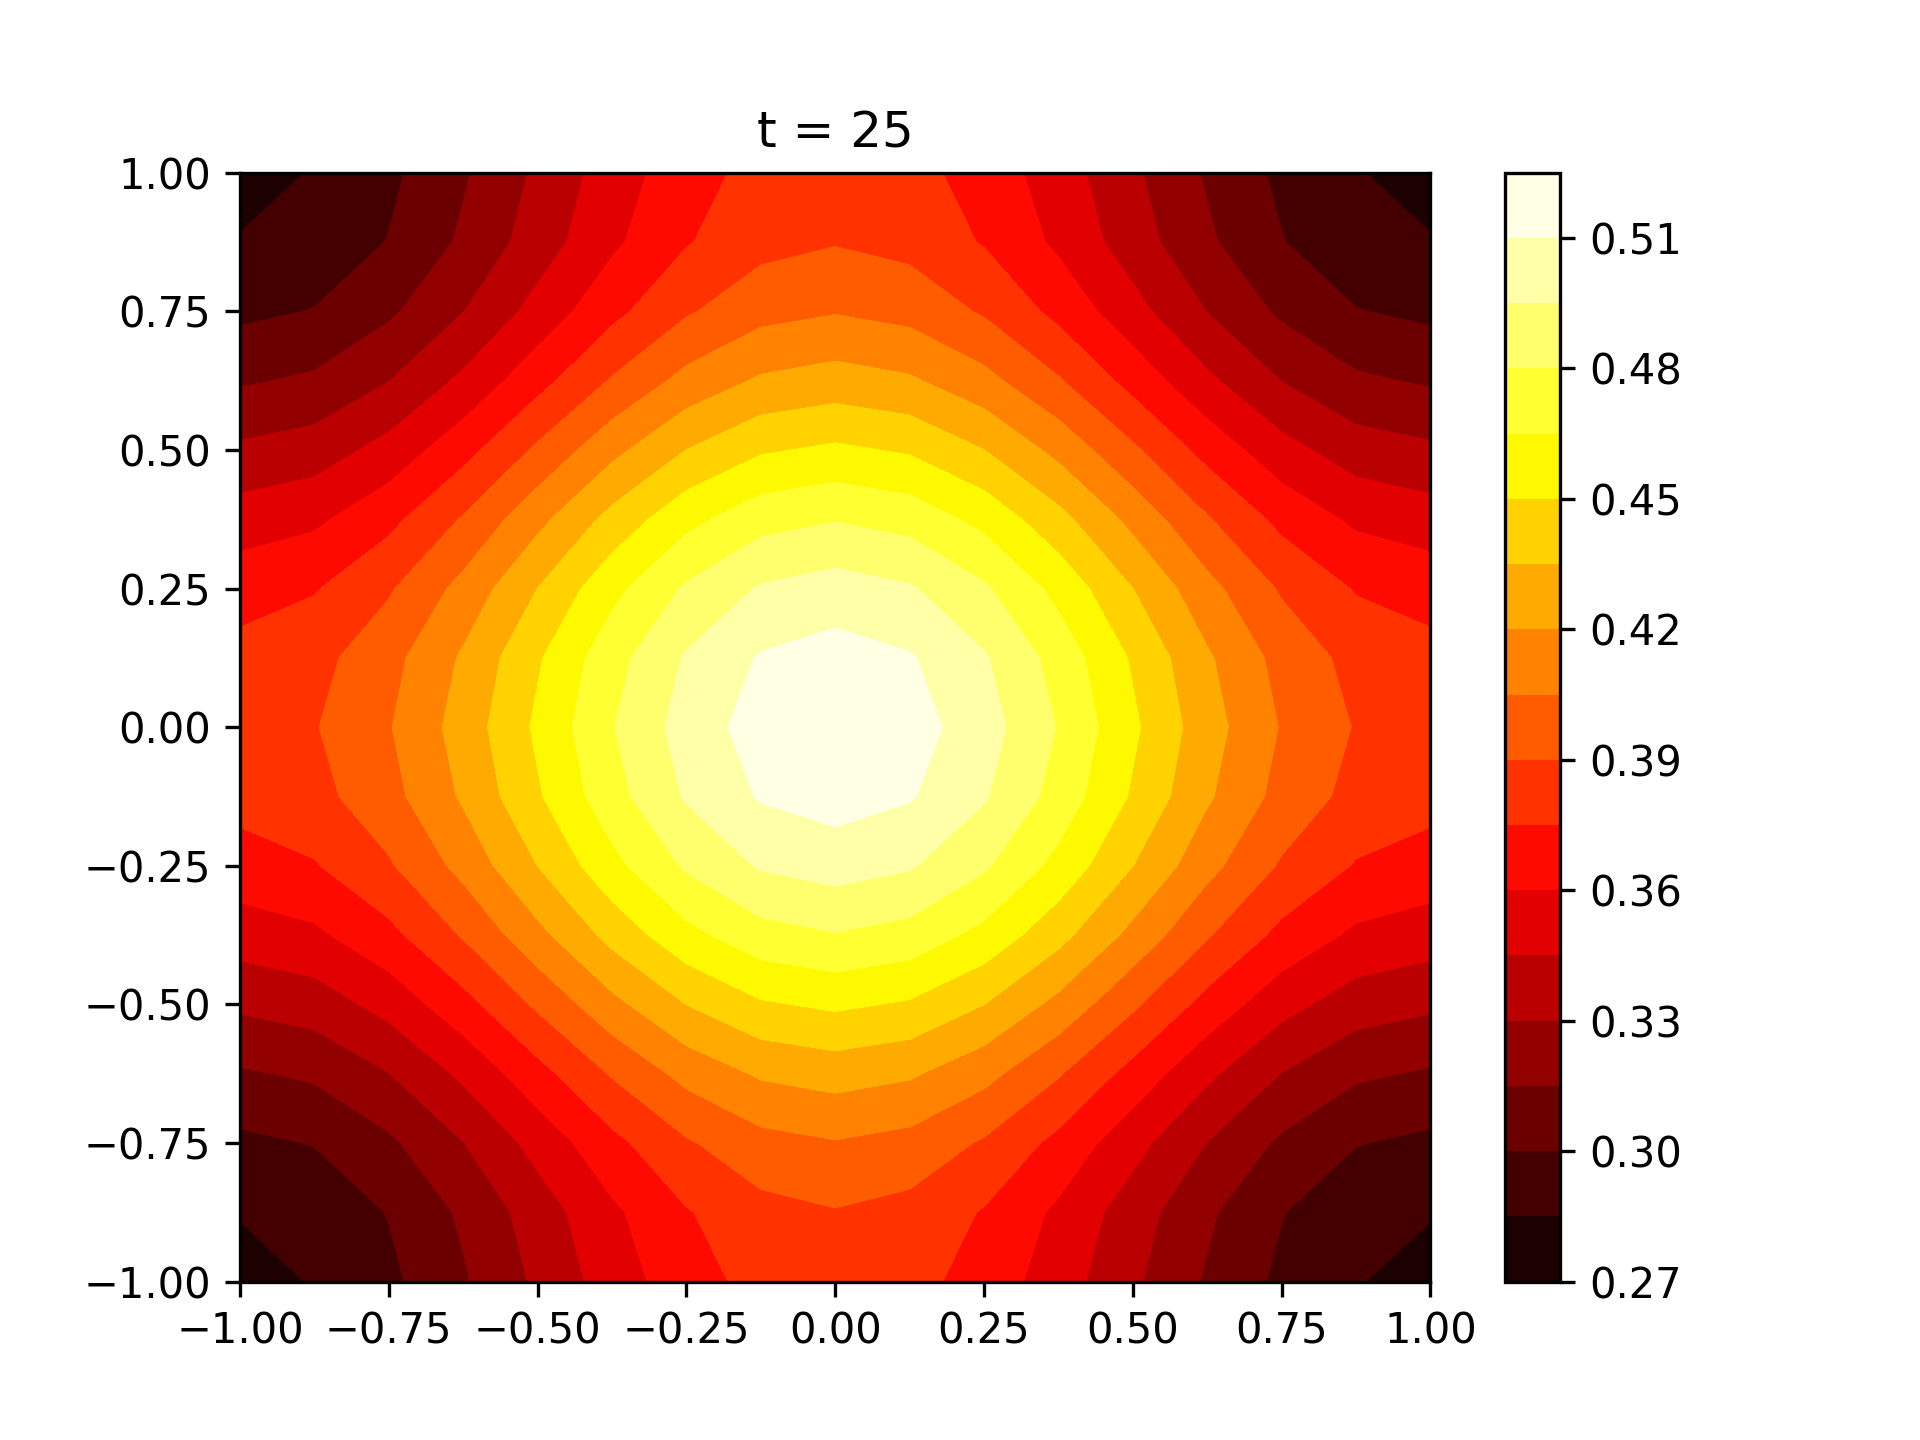
\includegraphics[width=\textwidth]{figs/q7a_heatmap_t25.png}
         \caption{$T=25~s$, solução explícita}
	\label{fig:q7a_heatmap_t25}
     \end{subfigure}
     \hfill
     \begin{subfigure}[b]{0.49\textwidth}
         \centering
     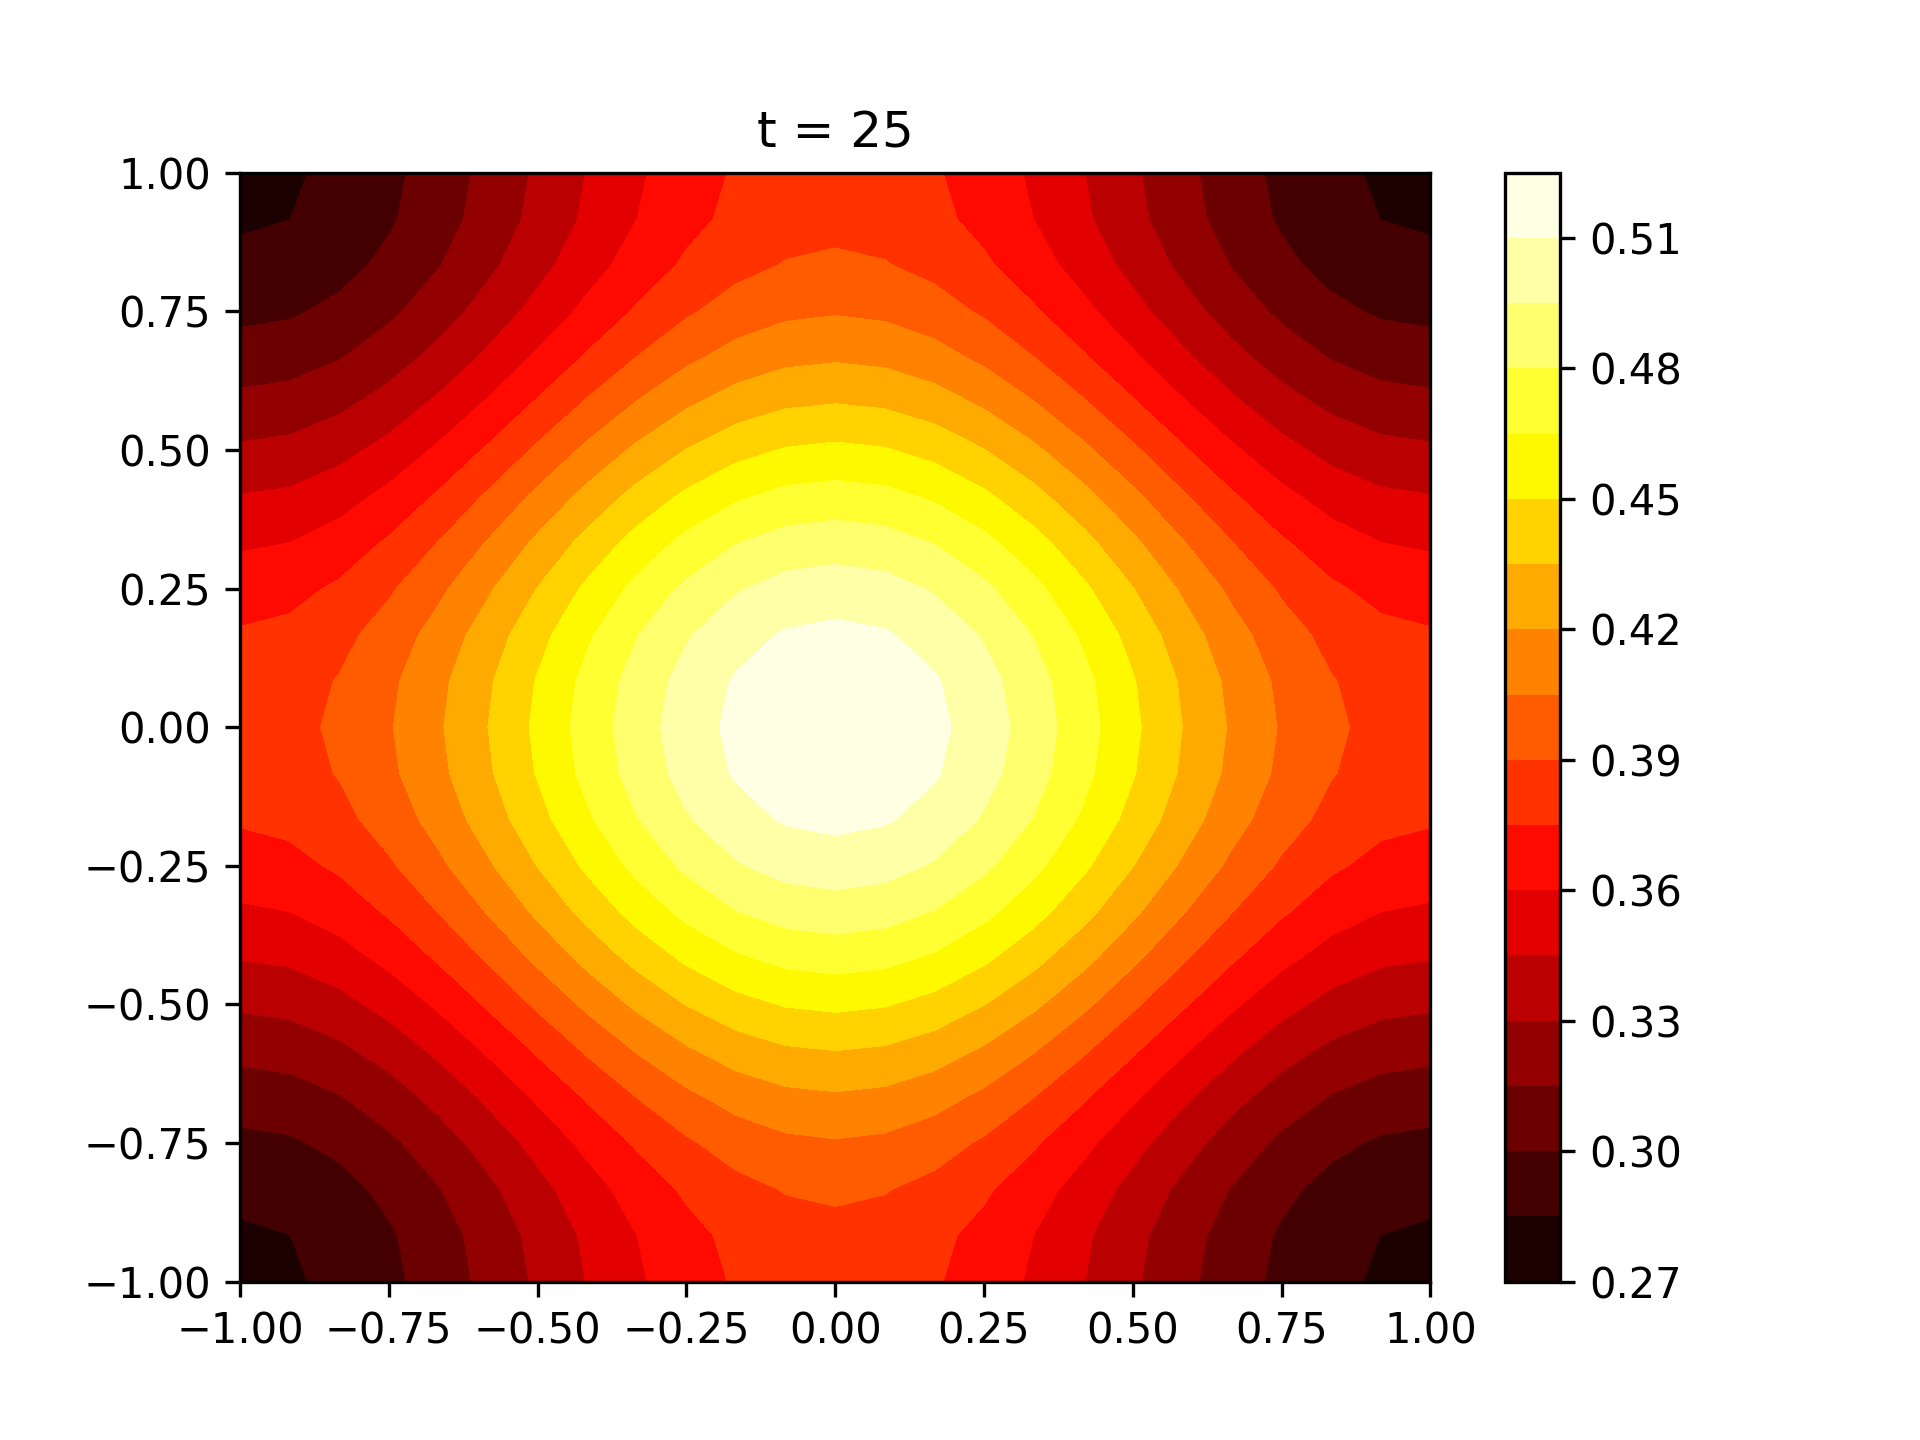
\includegraphics[width=\textwidth]{figs/q7b_heatmap_t25.png}
         \caption{$T=25~s$, solução implícita}
	\label{fig:q7b_heatmap_t25}
     \end{subfigure}
     \vfill
     \begin{subfigure}[b]{0.49\textwidth}
         \centering
         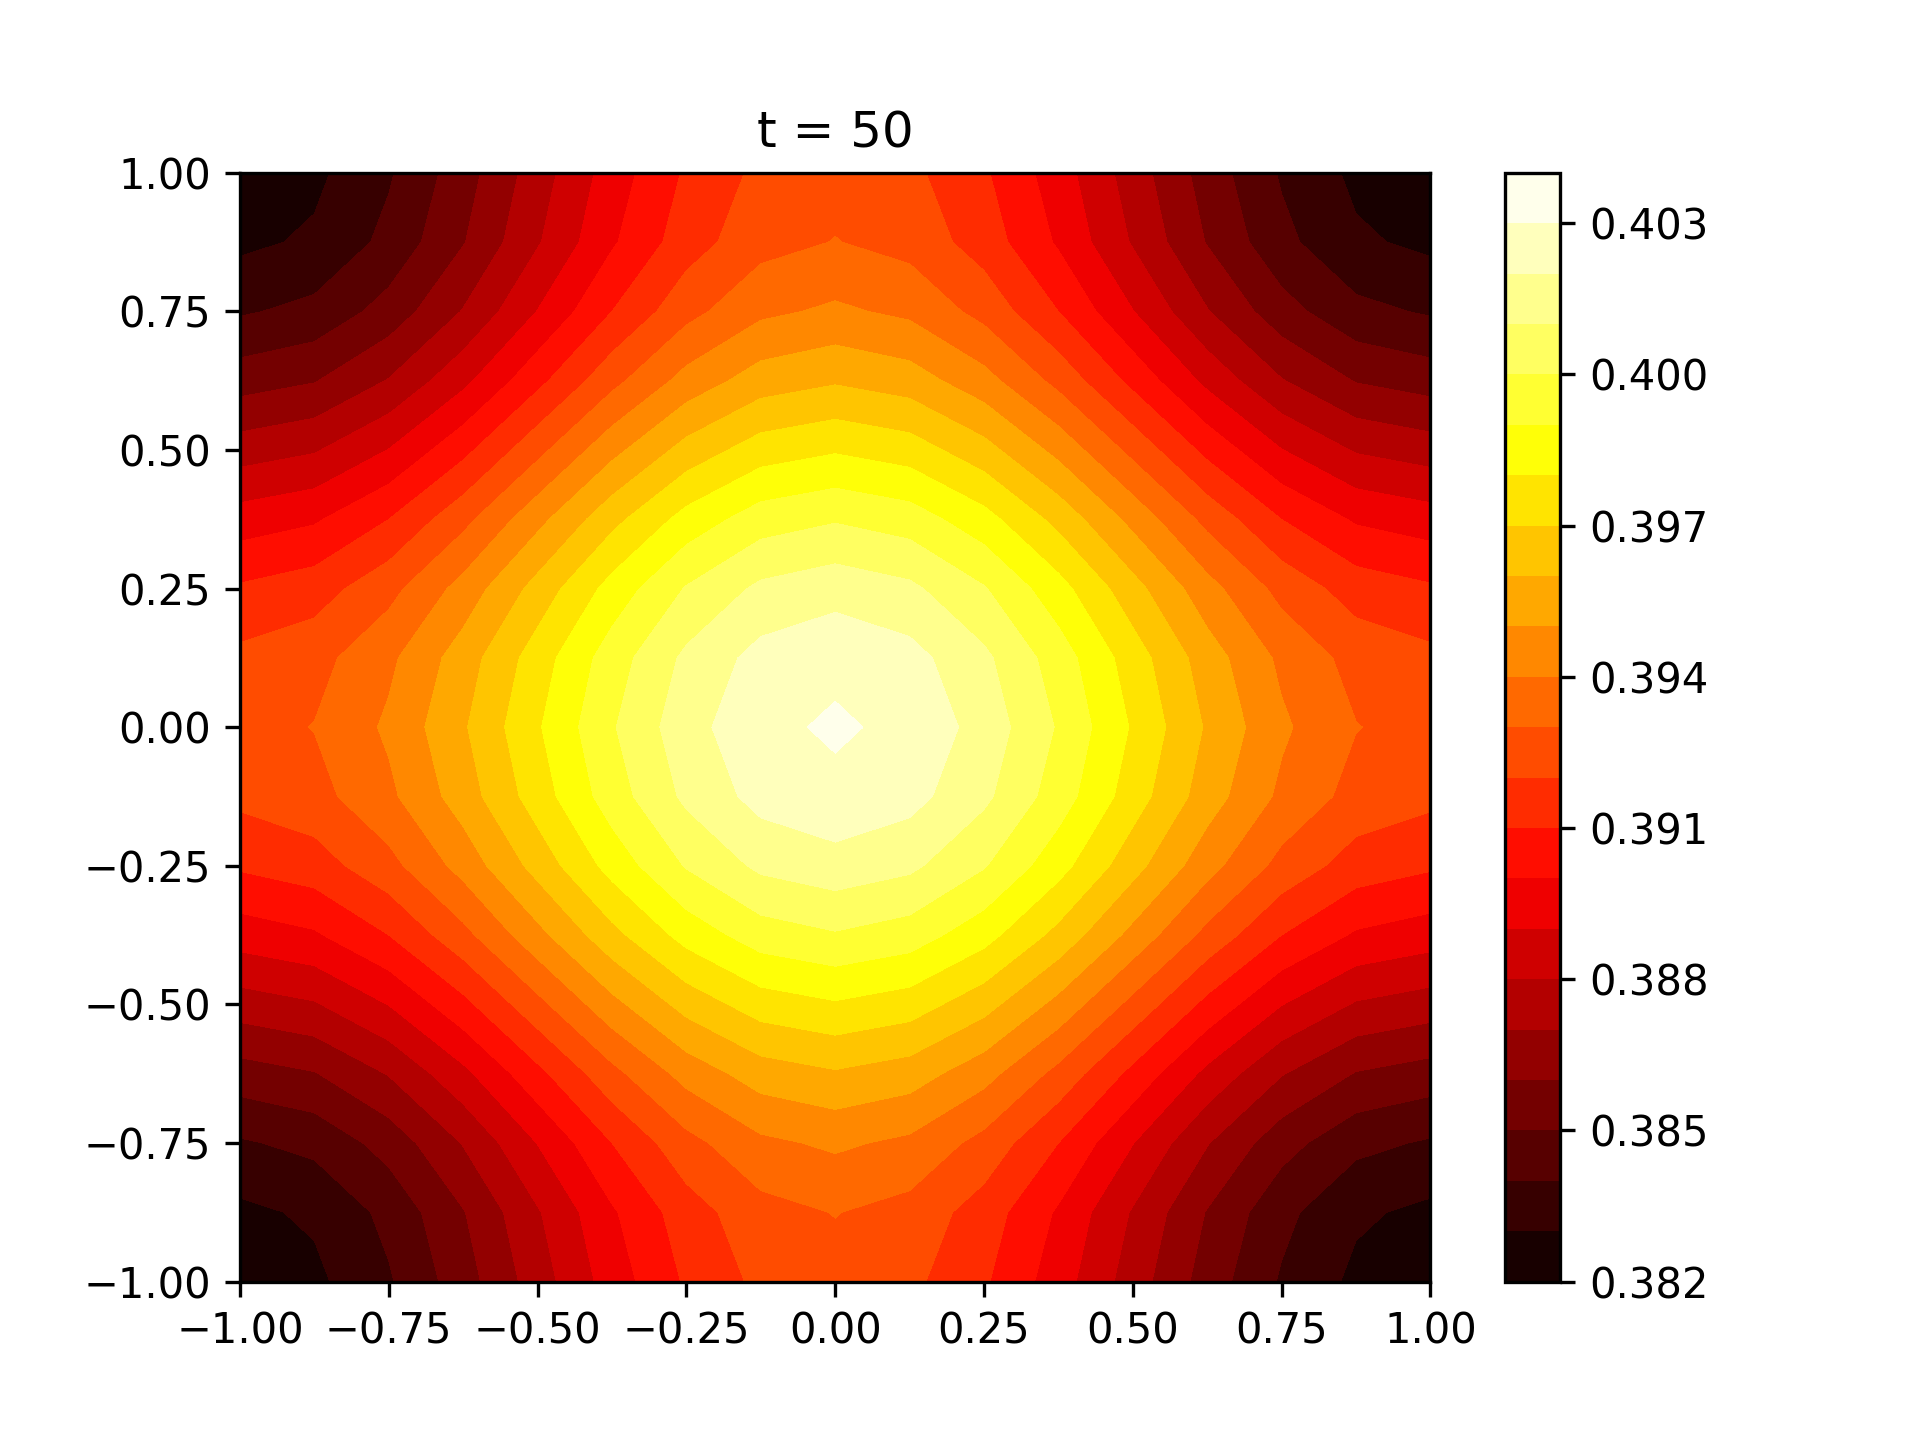
\includegraphics[width=\textwidth]{figs/q7a_heatmap_t50.png}
         \caption{$T=50~s$, solução explícita}
	\label{fig:q7a_heatmap_t50}
     \end{subfigure}
     \hfill
     \begin{subfigure}[b]{0.49\textwidth}
         \centering
     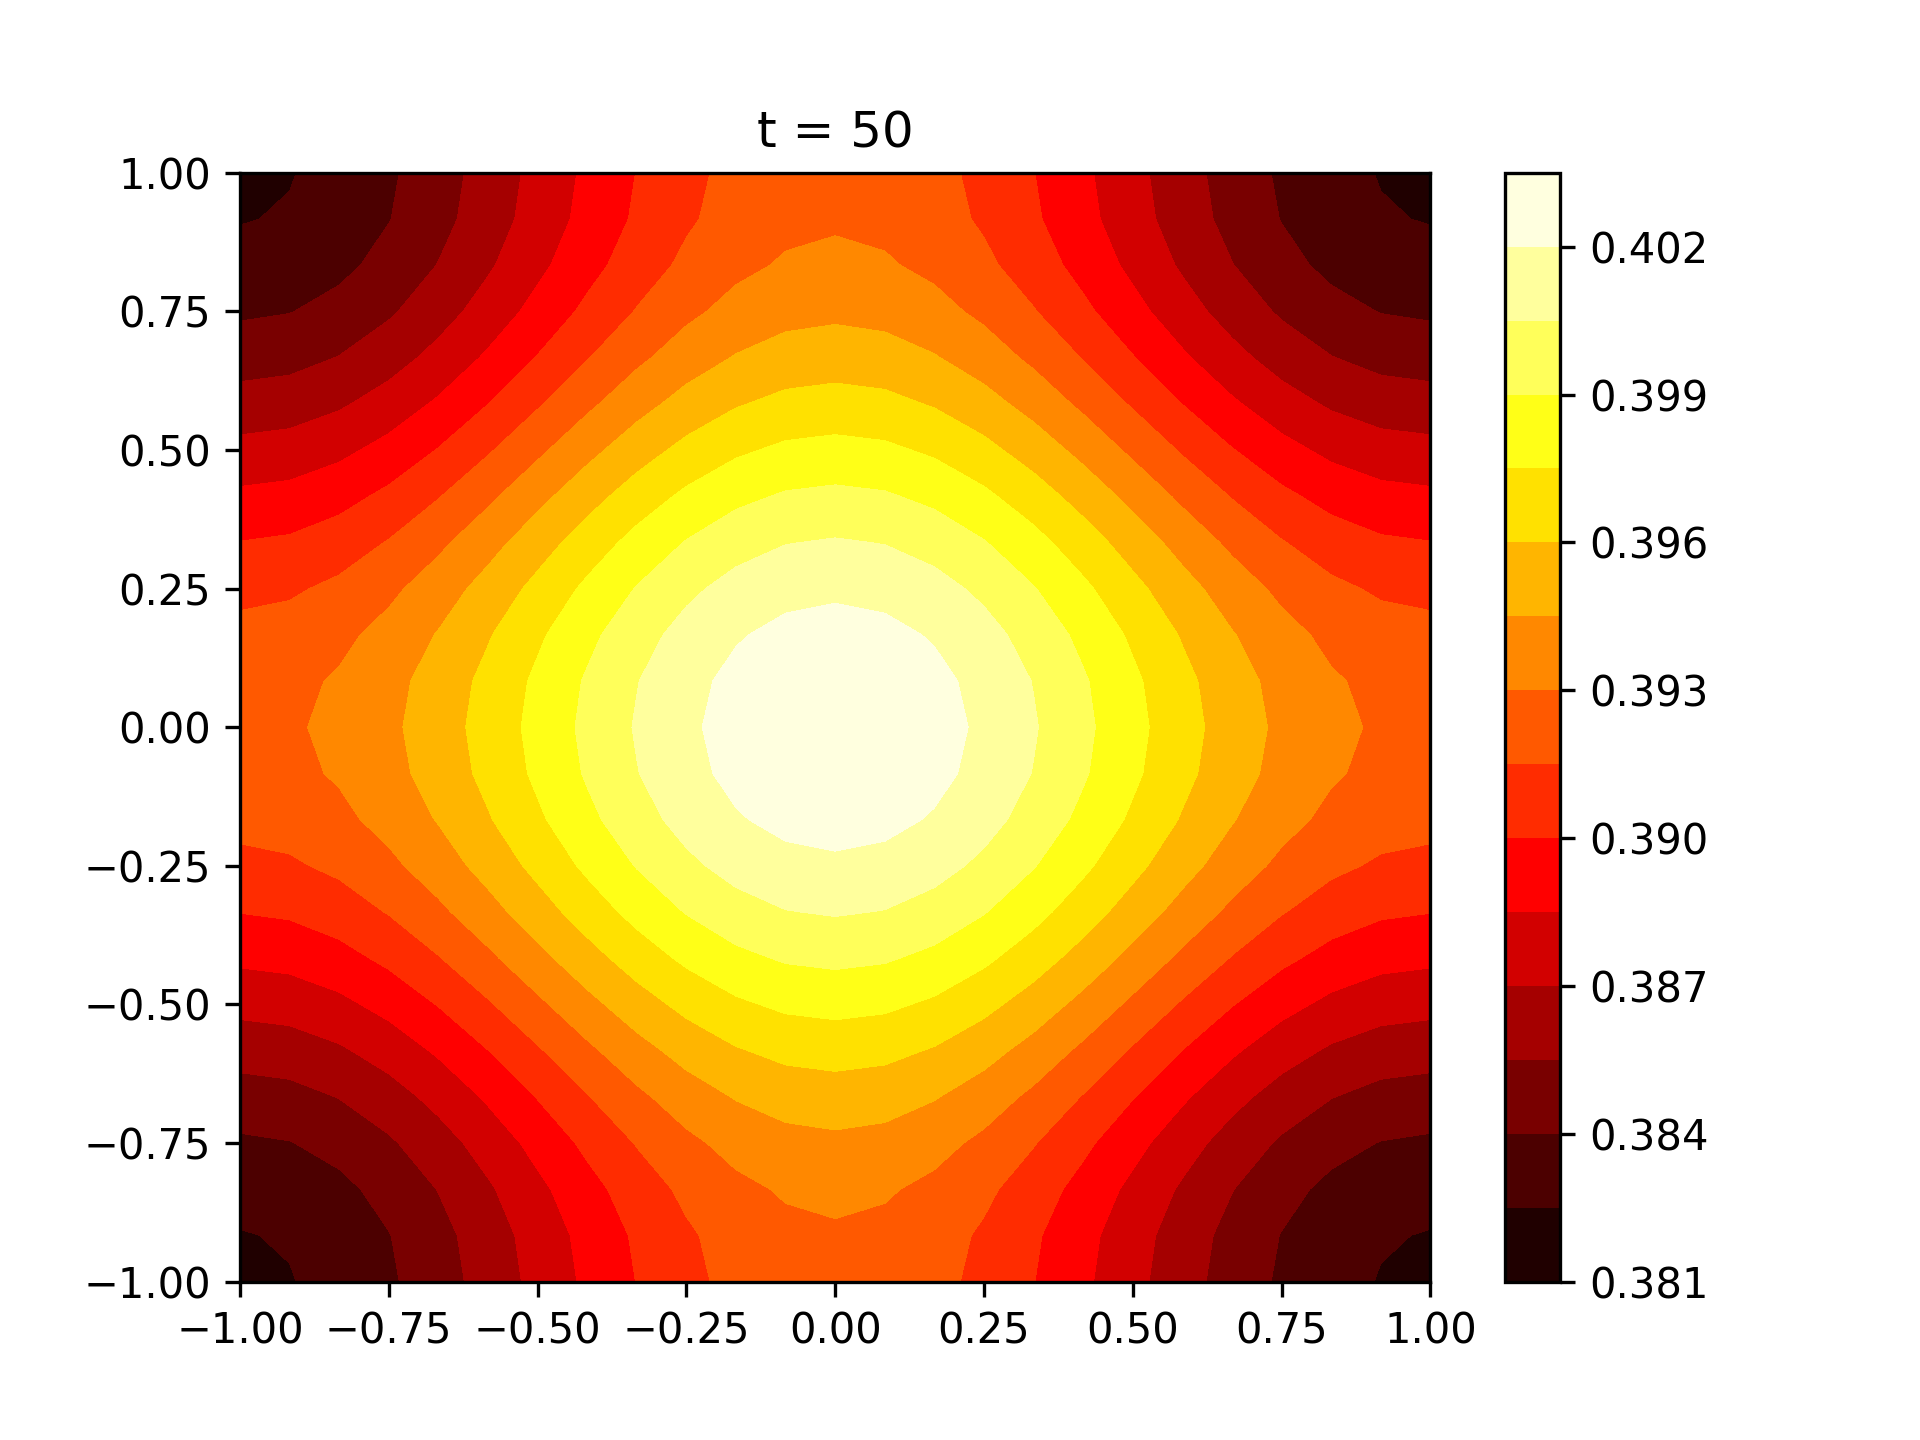
\includegraphics[width=\textwidth]{figs/q7b_heatmap_t50.png}
         \caption{$T=50~s$, solução implícita}
	\label{fig:q7b_heatmap_t50}
     \end{subfigure}
     \begin{subfigure}[b]{0.49\textwidth}
         \centering
         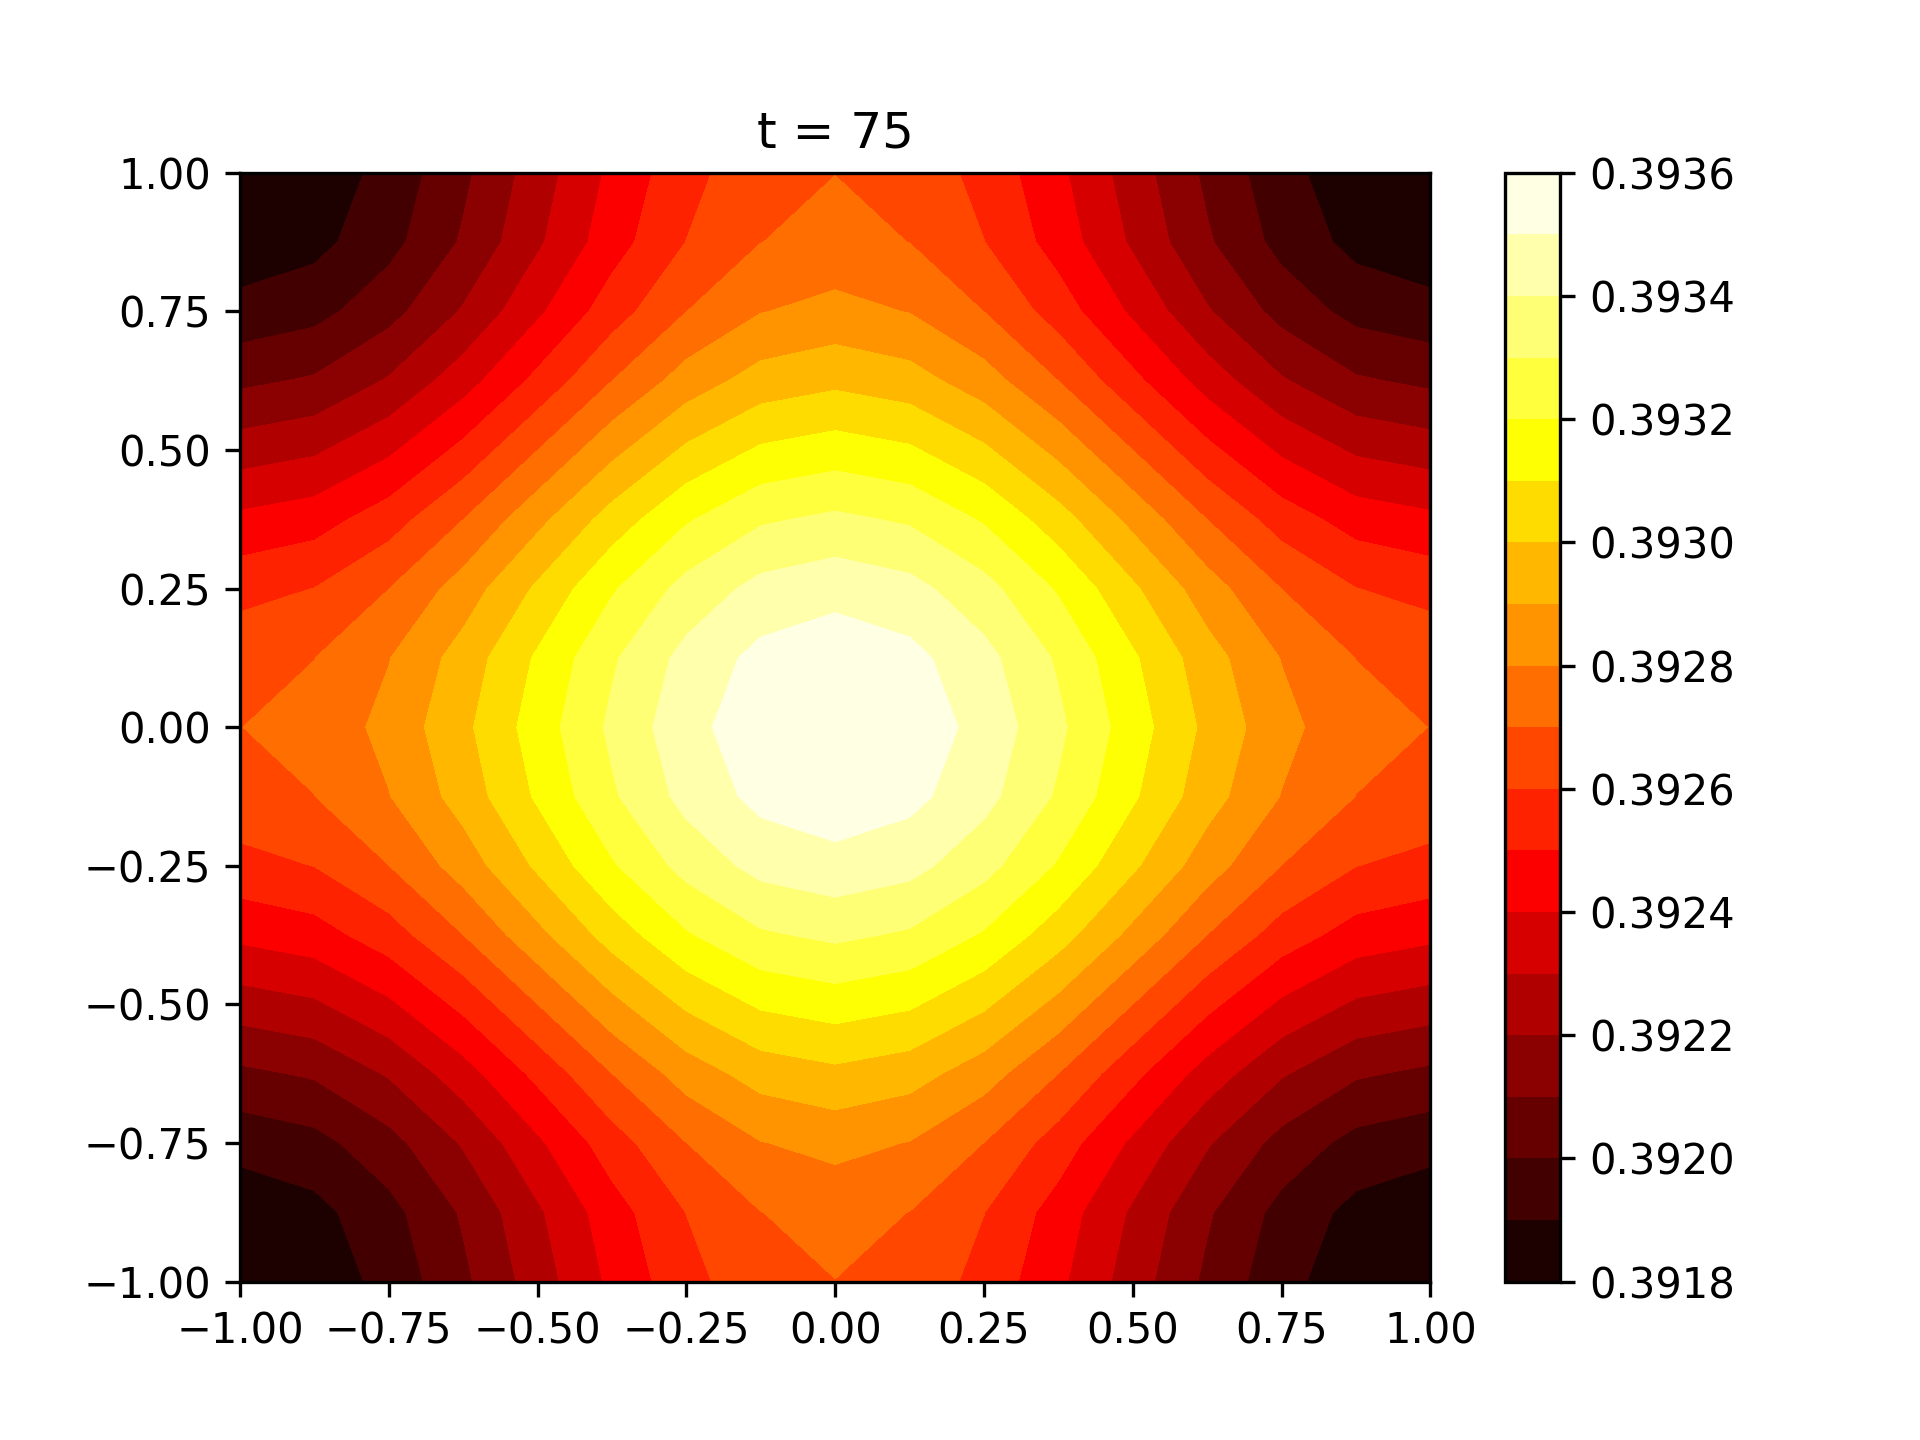
\includegraphics[width=\textwidth]{figs/q7a_heatmap_t75.png}
         \caption{$T=75~s$, solução explícita}
	\label{fig:q7a_heatmap_t75}
     \end{subfigure}
     \hfill
     \begin{subfigure}[b]{0.49\textwidth}
         \centering
     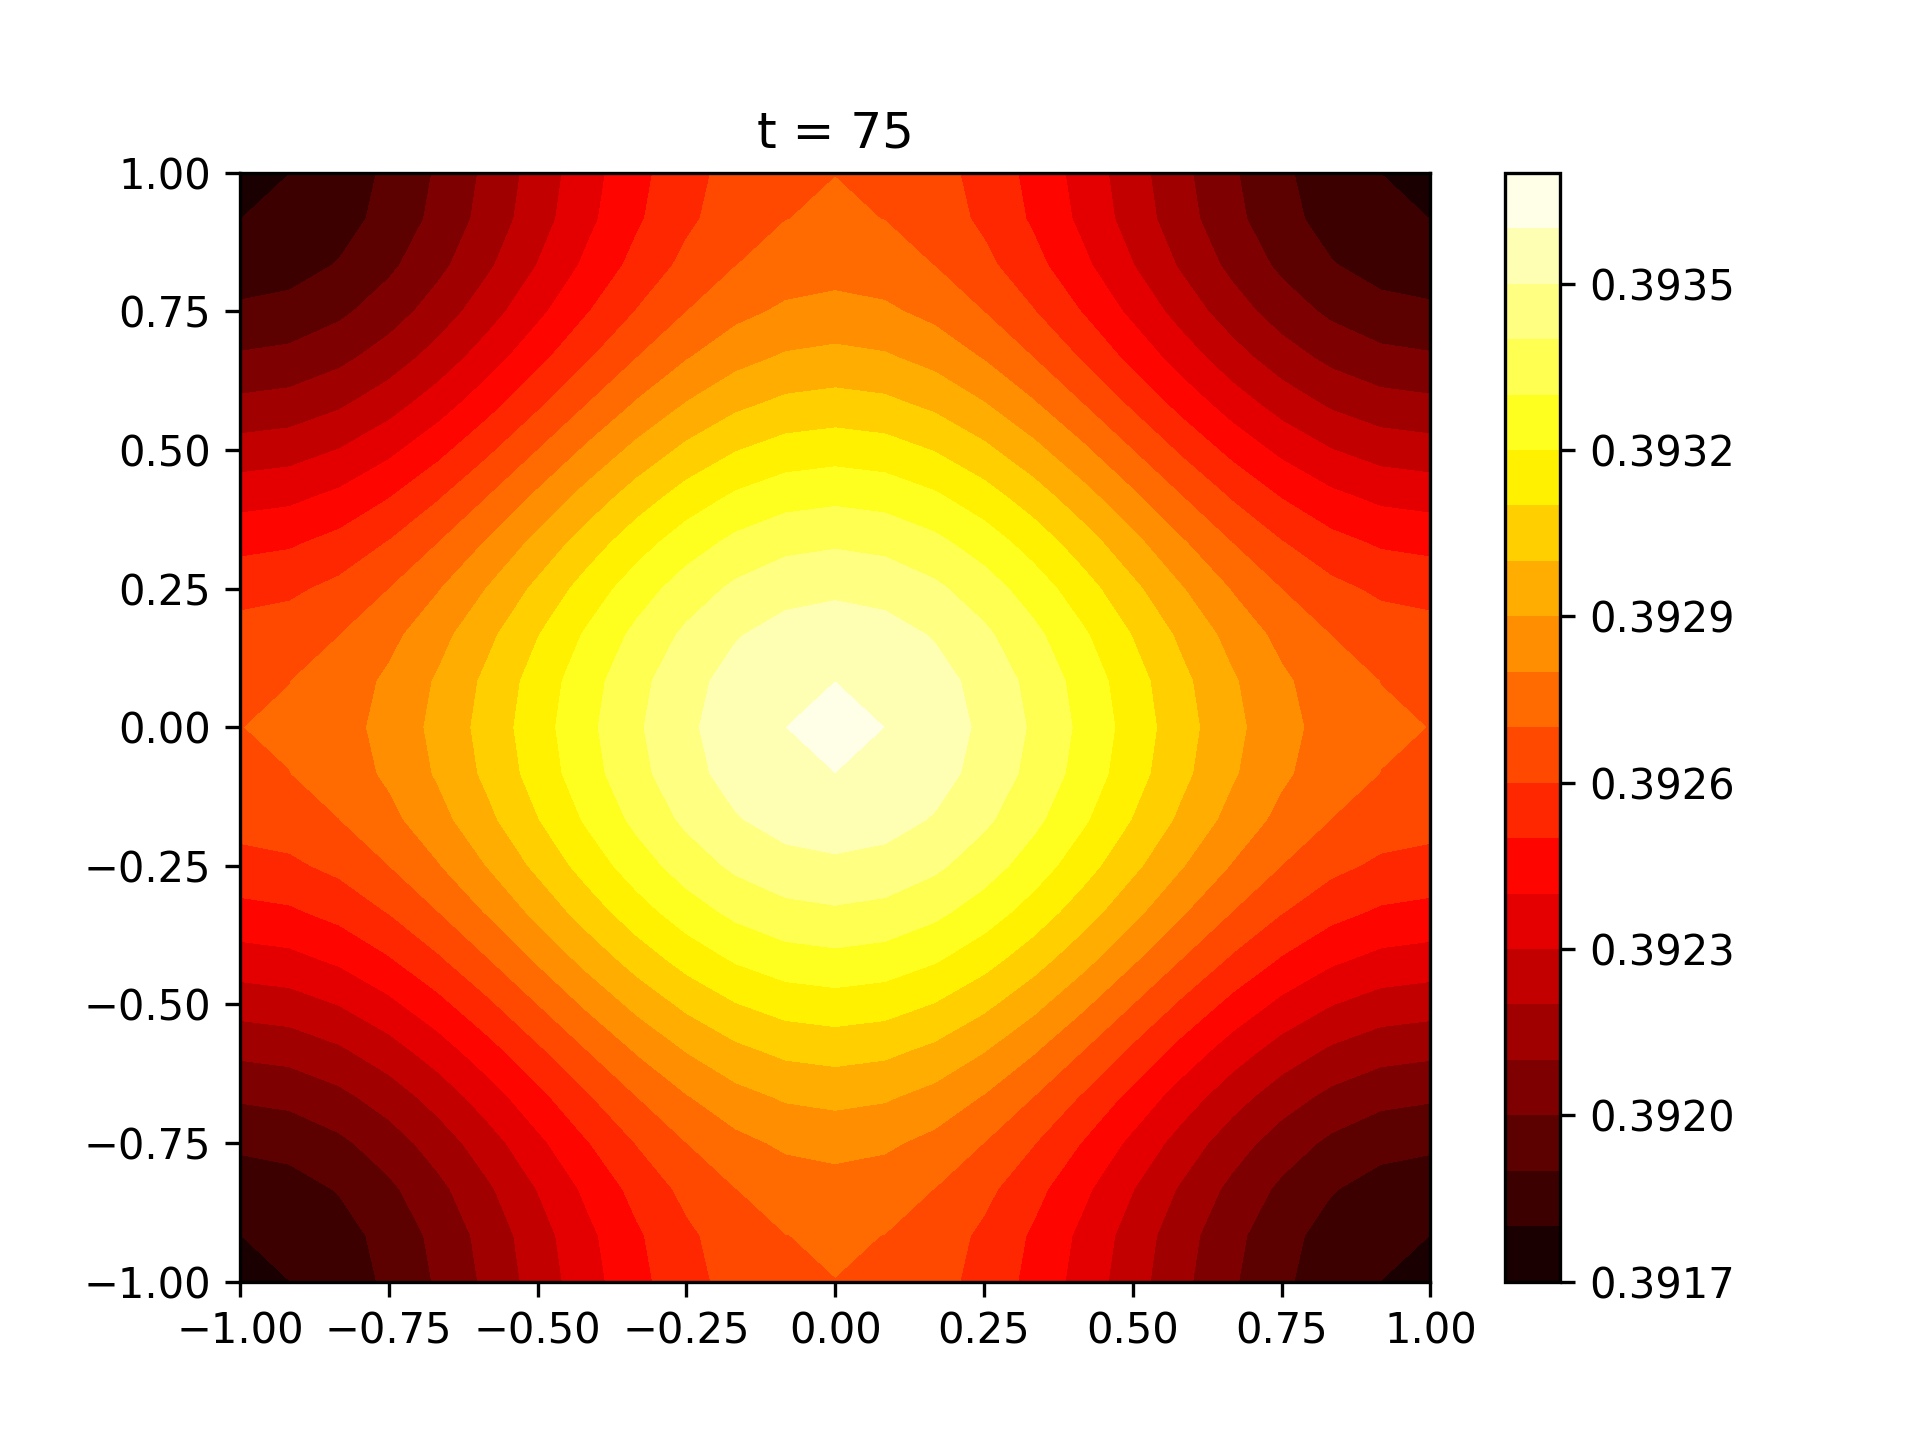
\includegraphics[width=\textwidth]{figs/q7b_heatmap_t75.png}
         \caption{$T=75~s$, solução implícita}
	\label{fig:q7b_heatmap_t75}
     \end{subfigure}
     \begin{subfigure}[b]{0.49\textwidth}
         \centering
         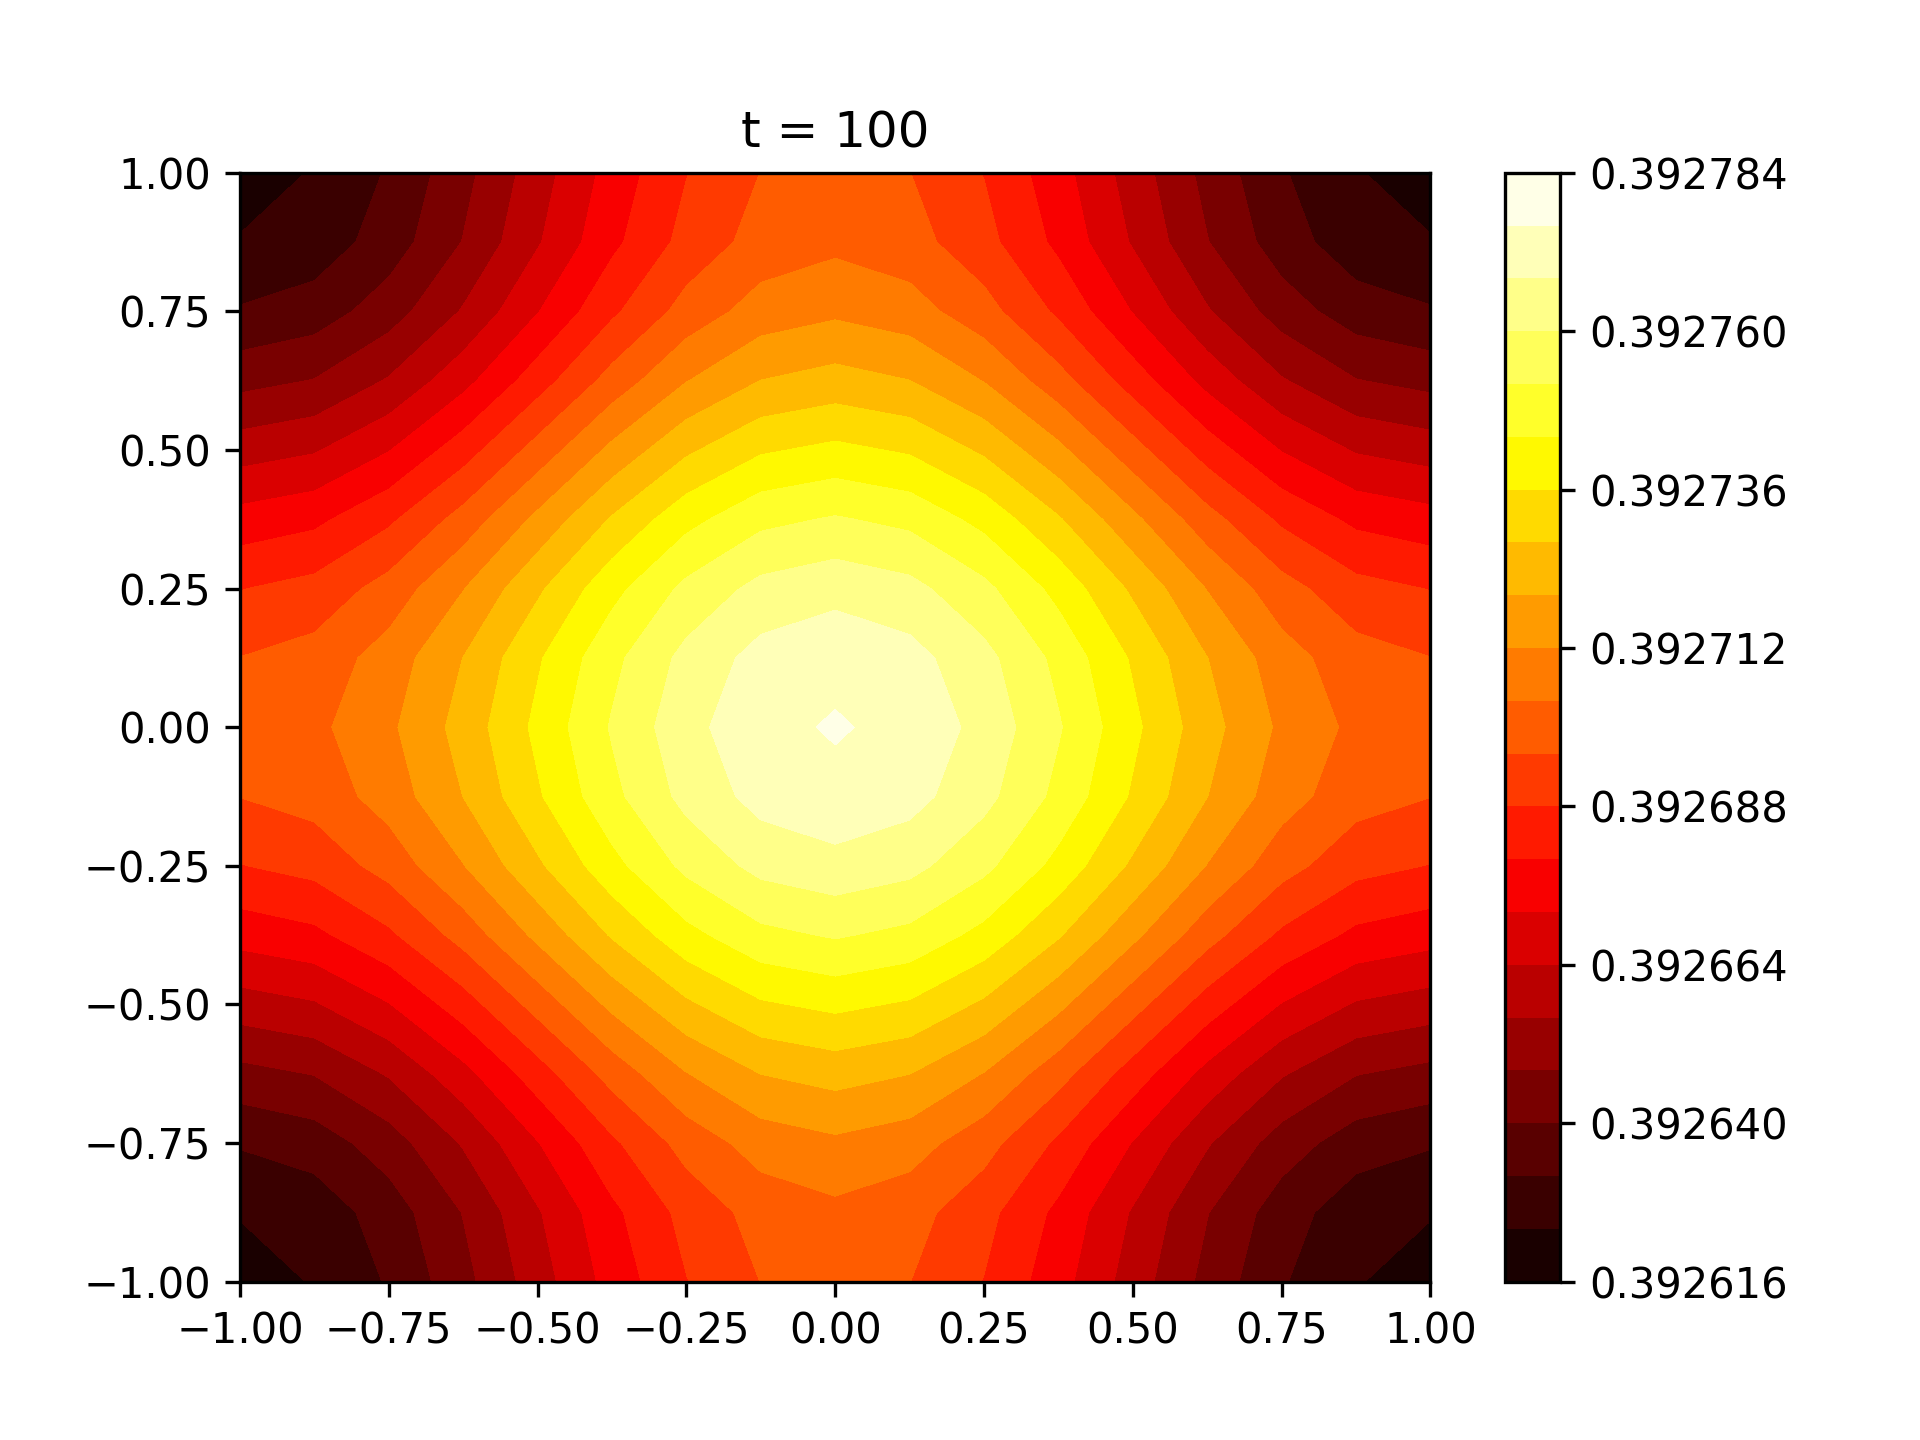
\includegraphics[width=\textwidth]{figs/q7a_heatmap_t100.png}
         \caption{$T=100~s$, solução explícita}
	\label{fig:q7a_heatmap_t100}
     \end{subfigure}
     \hfill
     \begin{subfigure}[b]{0.49\textwidth}
         \centering
     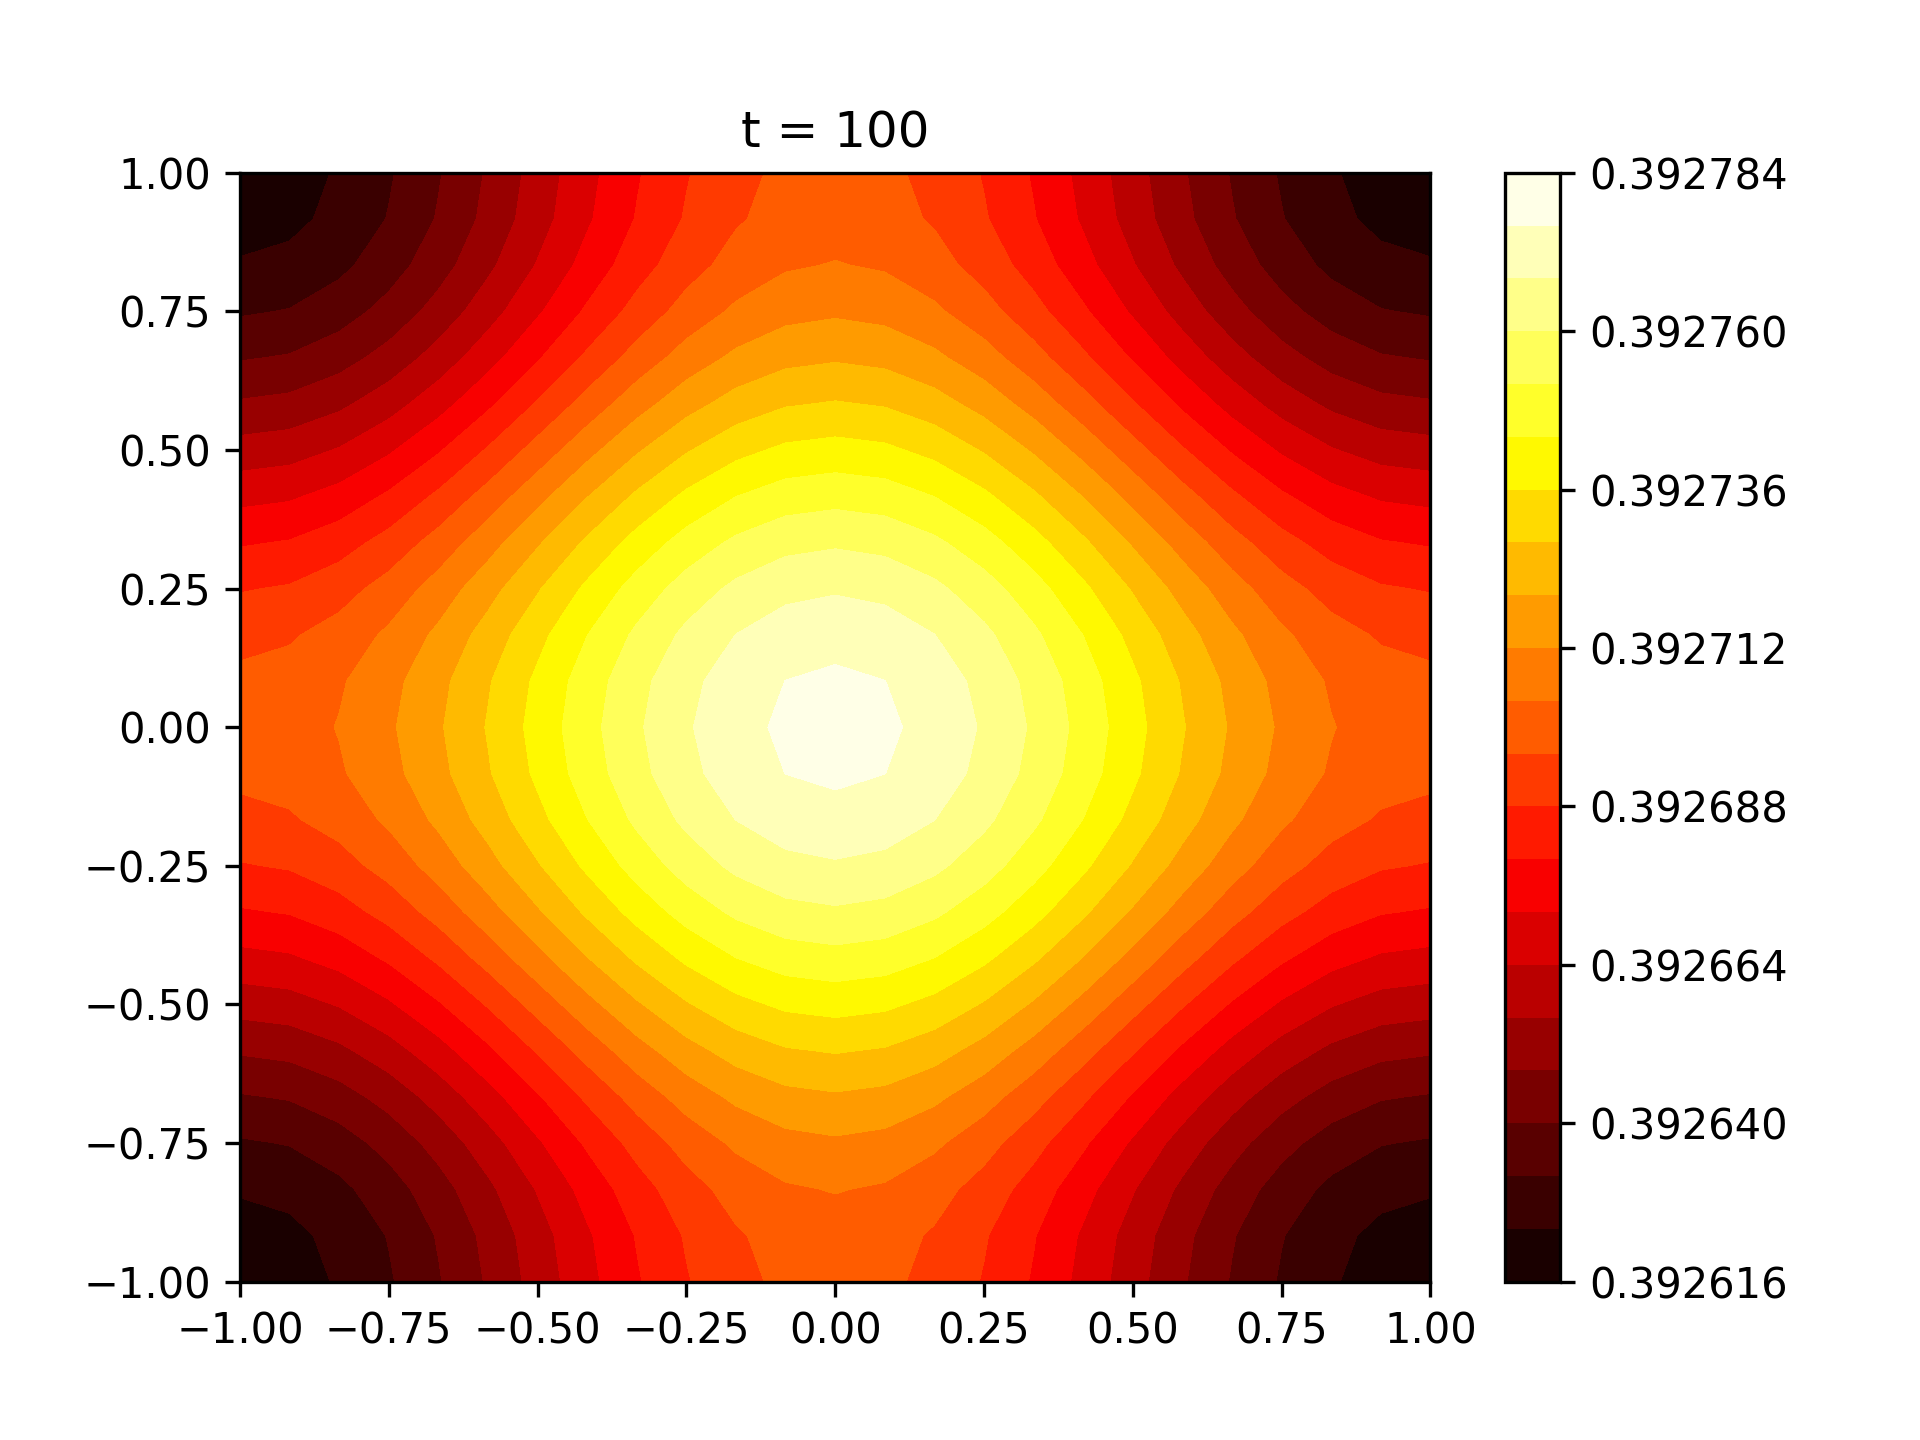
\includegraphics[width=\textwidth]{figs/q7b_heatmap_t100.png}
         \caption{$T=100~s$, solução implícita}
	\label{fig:q7b_heatmap_t100}
     \end{subfigure}
\caption{Distribuição de temperatura em evoluindo em função do tempo para a Questão 7.}
\end{figure}

\begin{figure}[h]
\centering
     \begin{subfigure}[b]{0.49\textwidth}
         \centering
         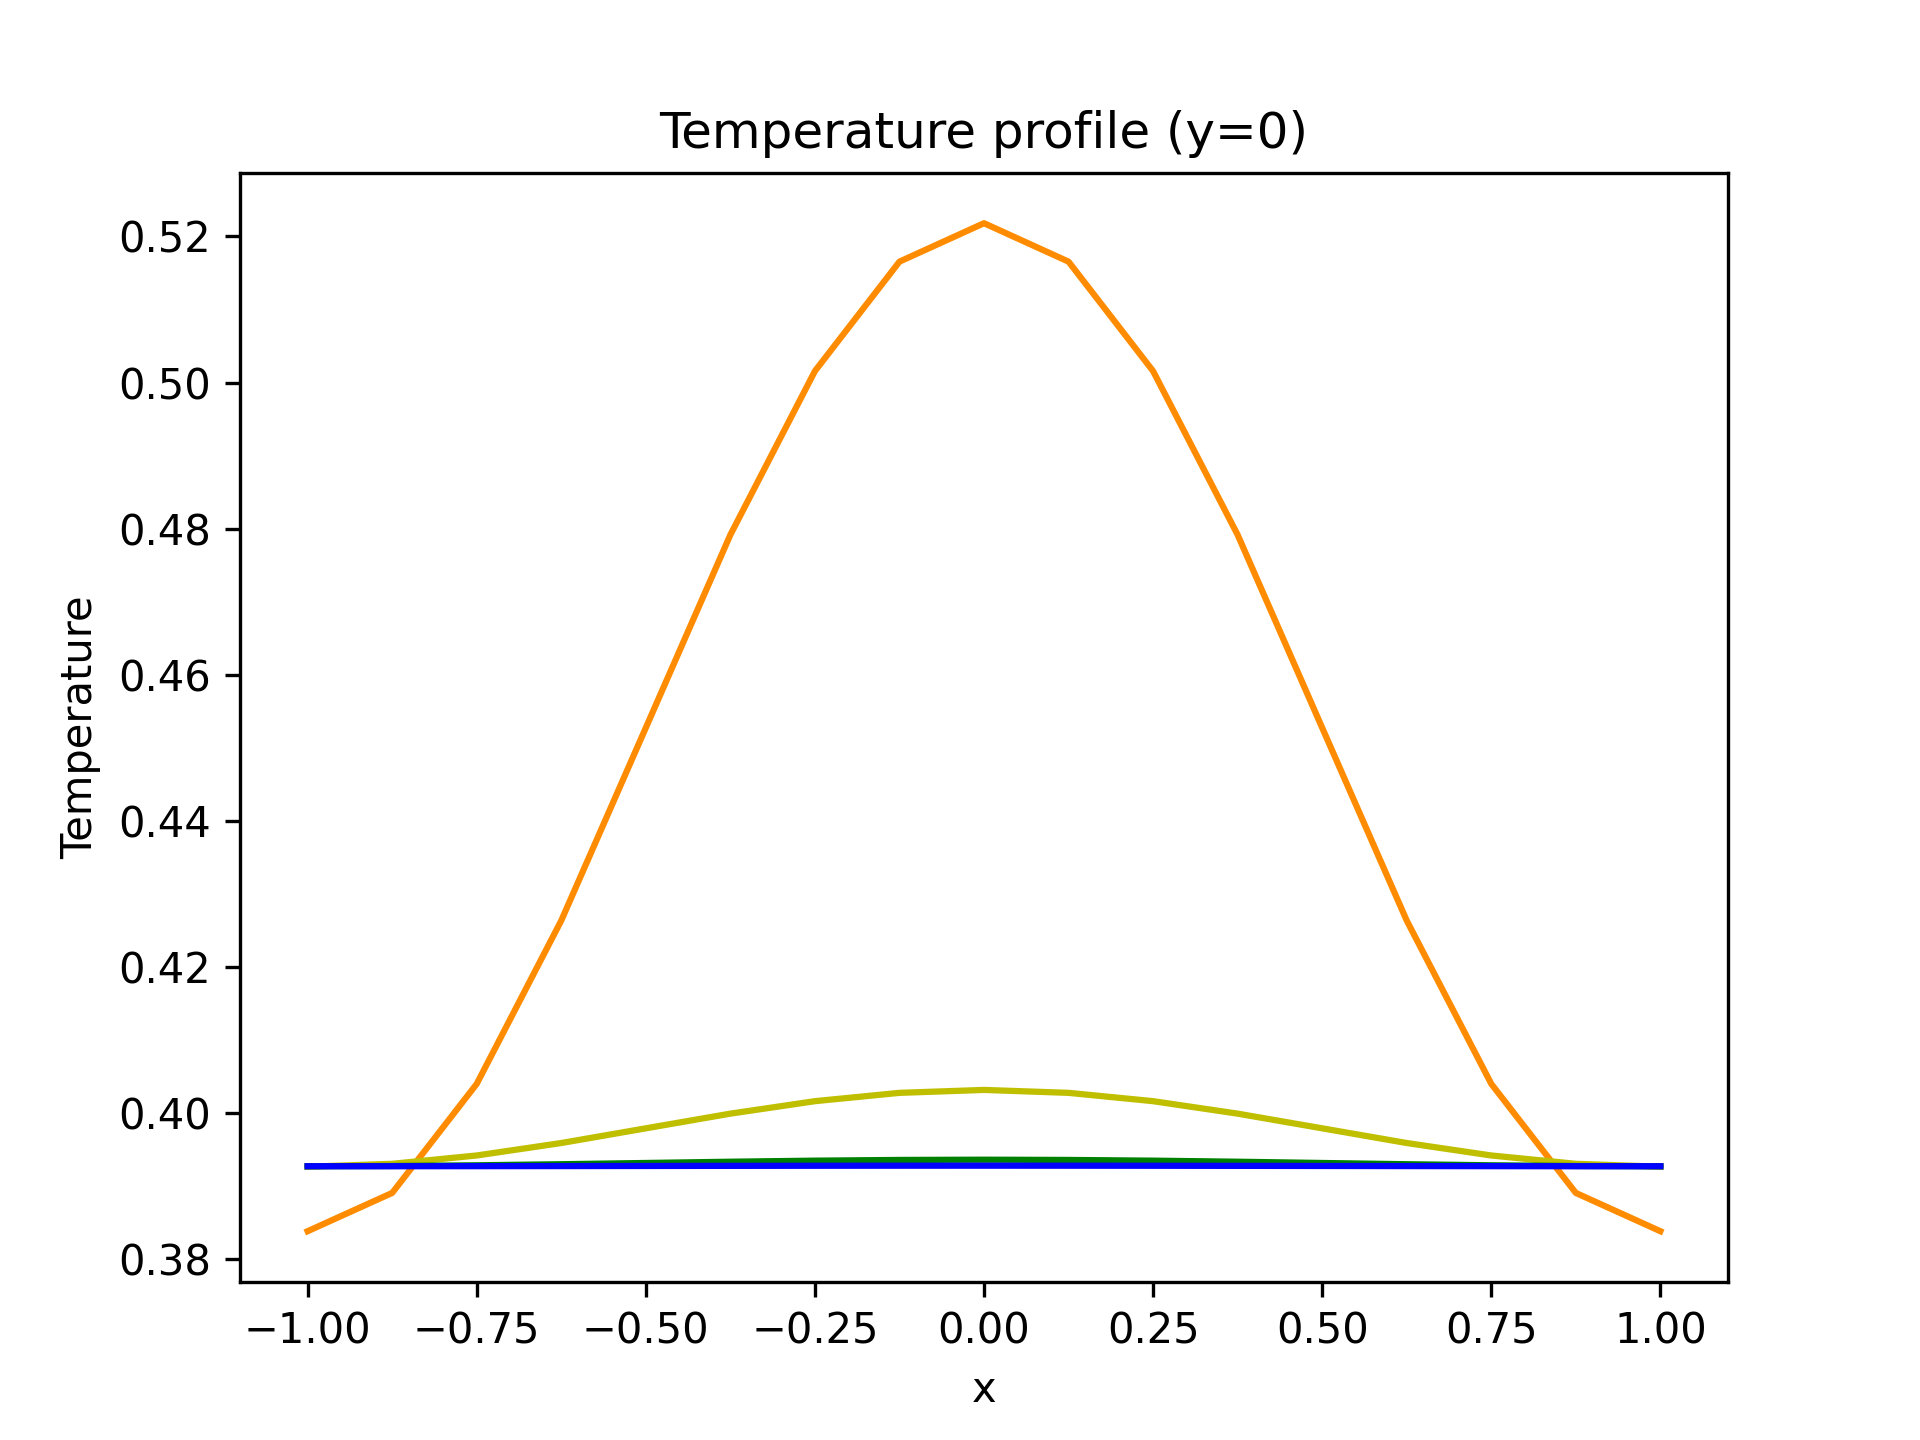
\includegraphics[width=\textwidth]{figs/q7a_temperature_profile.png}
         \caption{solução explícita}
	\label{fig:q7a_temperature_profile}
     \end{subfigure}
     \hfill
     \begin{subfigure}[b]{0.49\textwidth}
         \centering
     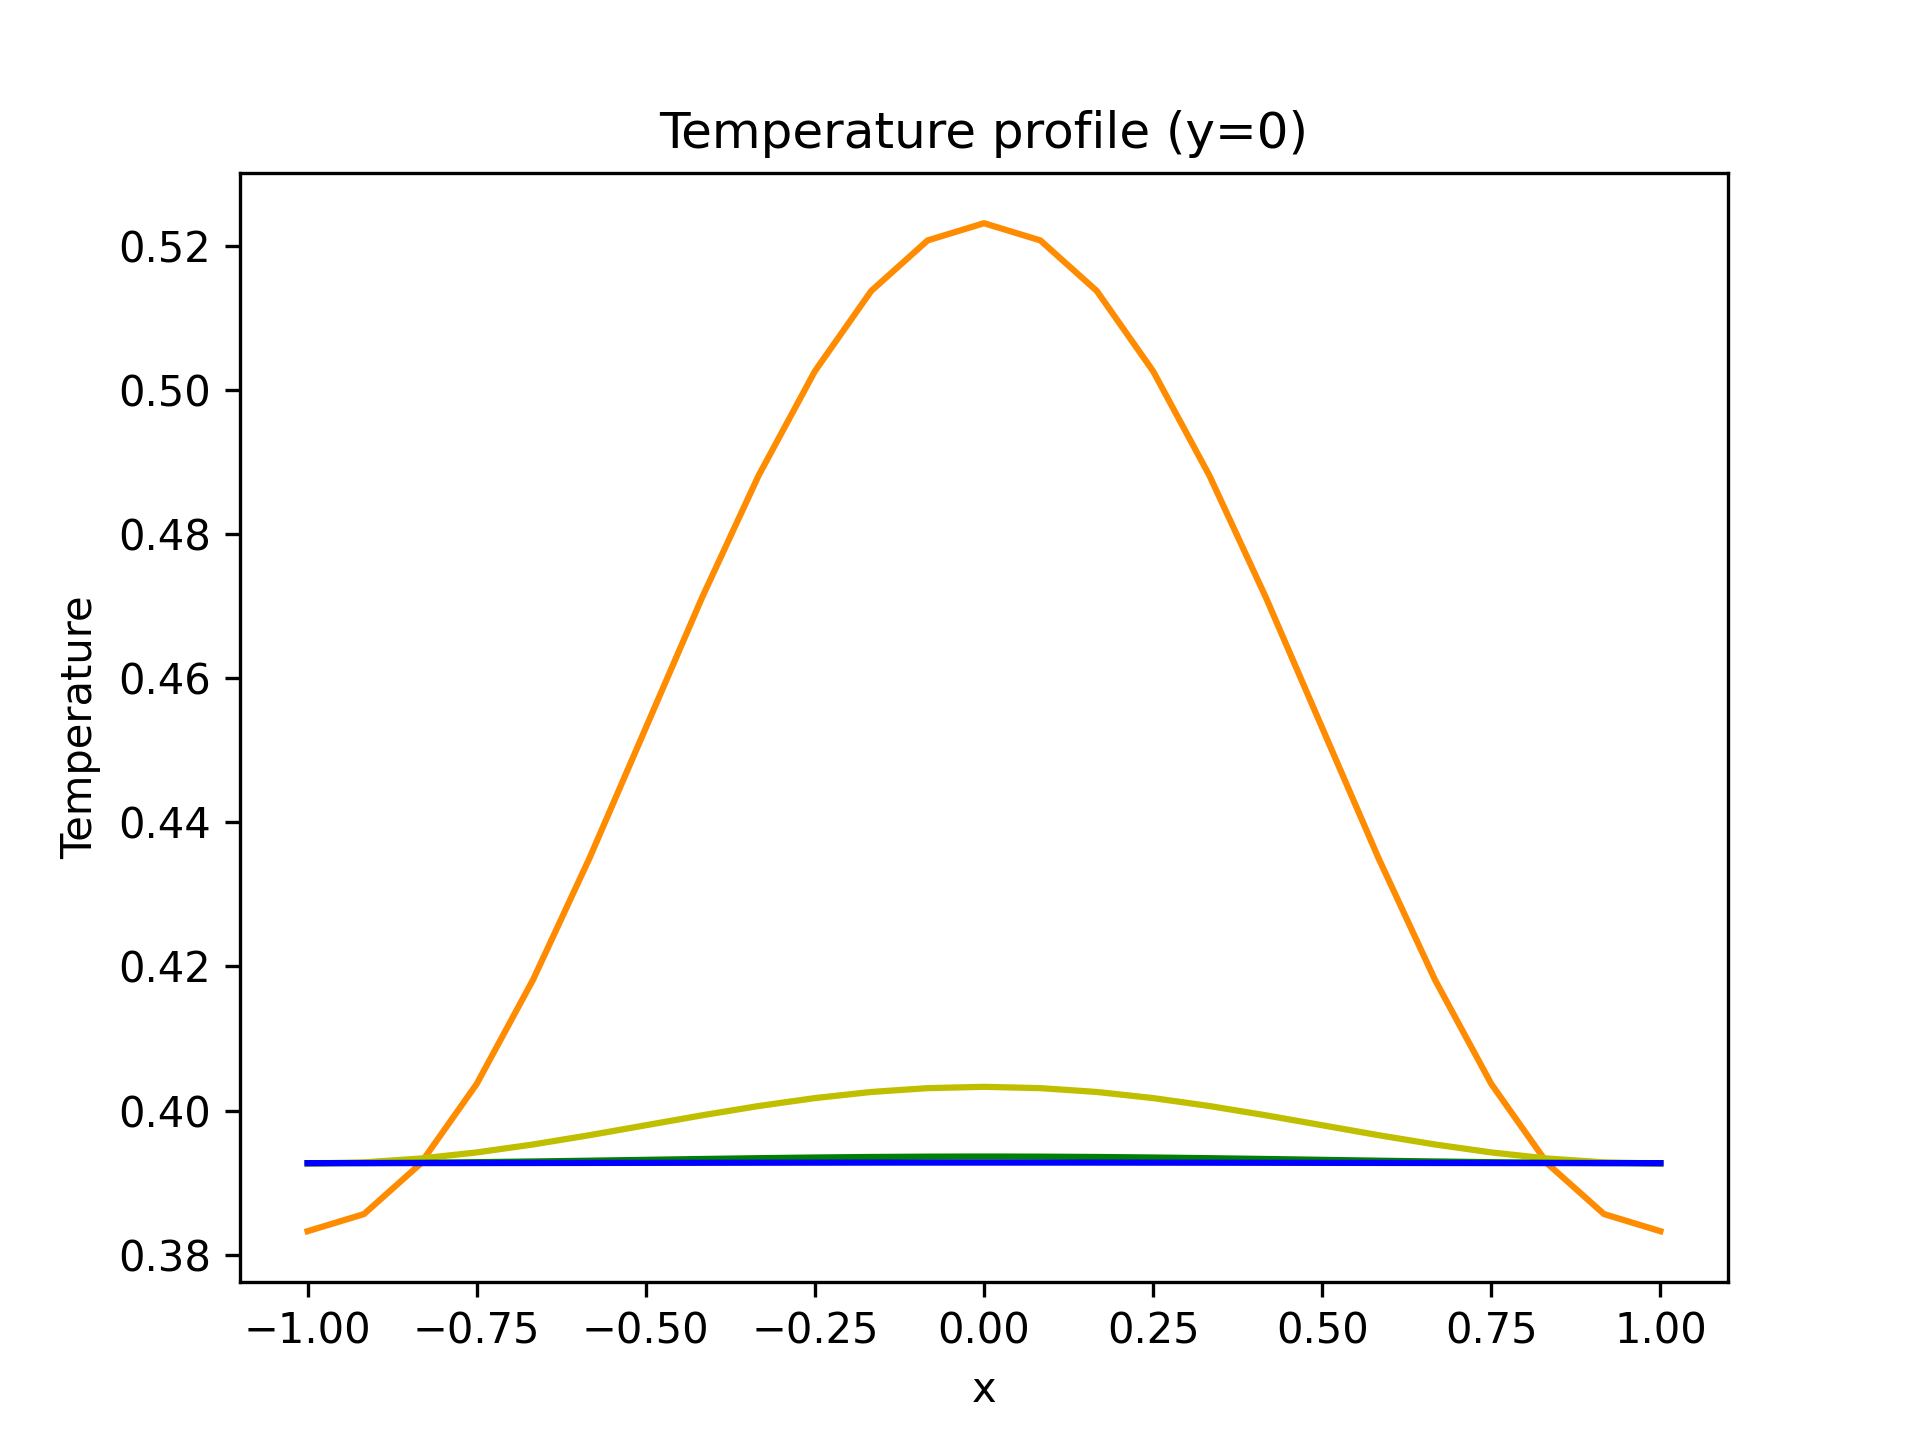
\includegraphics[width=\textwidth]{figs/q7b_temperature_profile.png}
         \caption{solução implícita}
	\label{fig:q7b_temperature_profile}
     \end{subfigure}
	\caption{Perfis de temperatura para questão 7.}
\end{figure}



\begin{thebibliography}{9}
\bibitem{leveque}
Randall J. LeVeque (2007) \emph{Finite Difference Methods for Ordinary and Partial Differential Equations:
Steady-State and Time-Dependent Problems}, Society for Industrial and Applied Mathematics 

\bibitem{chinesta}
Francisco Chinesta, Amine Ammar, Adrien Leygue, Roland Keunings. An overview of the proper generalized decomposition with applications in computational rheology. Journal of Non-Newtonian Fluid Mechanics, 2011, 166 (11), pp.578-592. hal-01061441
\end{thebibliography}
\end{document}
